\documentclass[a4paper,12pt]{extarticle}
\usepackage{geometry}
\usepackage[T1]{fontenc}
\usepackage[utf8]{inputenc}
\usepackage[english,russian]{babel}
\usepackage{amsmath}
\usepackage{amsthm}
\usepackage{amssymb}
\usepackage{fancyhdr}
\usepackage{setspace}
\usepackage{graphicx}
\usepackage{colortbl}
\usepackage{tikz}
\usepackage{pgf}
\usepackage{subcaption}
\usepackage{listings}
\usepackage{indentfirst}
\usepackage[
backend=biber,
style=numeric,
maxbibnames=99
]{biblatex}
\addbibresource{refs.bib}
\usepackage[colorlinks,citecolor=blue,linkcolor=blue,bookmarks=false,hypertexnames=true, urlcolor=blue]{hyperref} 
\usepackage{indentfirst}
\usepackage{mathtools}
\usepackage{booktabs}
\usepackage[flushleft]{threeparttable}
\usepackage{tablefootnote}

\usepackage{chngcntr} % нумерация графиков и таблиц по секциям
\counterwithin{table}{section}
\counterwithin{figure}{section}

\graphicspath{{graphics/}}%путь к рисункам

\makeatletter
% \renewcommand{\@biblabel}[1]{#1.} % Заменяем библиографию с квадратных скобок на точку:
\makeatother

\geometry{left=2.5cm}% левое поле
\geometry{right=1.0cm}% правое поле
\geometry{top=2.0cm}% верхнее поле
\geometry{bottom=2.0cm}% нижнее поле
\setlength{\parindent}{1.25cm}
\renewcommand{\baselinestretch}{1.5} % междустрочный интервал


\newcommand{\bibref}[3]{\hyperlink{#1}{#2 (#3)}} % biblabel, authors, year
\addto\captionsrussian{\def\refname{Список литературы (или источников)}} 

\renewcommand{\theenumi}{\arabic{enumi}}% Меняем везде перечисления на цифра.цифра
\renewcommand{\labelenumi}{\arabic{enumi}}% Меняем везде перечисления на цифра.цифра
\renewcommand{\theenumii}{.\arabic{enumii}}% Меняем везде перечисления на цифра.цифра
\renewcommand{\labelenumii}{\arabic{enumi}.\arabic{enumii}.}% Меняем везде перечисления на цифра.цифра
\renewcommand{\theenumiii}{.\arabic{enumiii}}% Меняем везде перечисления на цифра.цифра
\renewcommand{\labelenumiii}{\arabic{enumi}.\arabic{enumii}.\arabic{enumiii}.}% Меняем везде перечисления на цифра.цифра

\begin{document}
\begin{titlepage}
\newpage

{\setstretch{1.0}
\begin{center}
ПРАВИТЕЛЬСТВО РОССИЙСКОЙ ФЕДЕРАЦИИ\\
ФГАОУ ВО НАЦИОНАЛЬНЫЙ ИССЛЕДОВАТЕЛЬСКИЙ УНИВЕРСИТЕТ\\
«ВЫСШАЯ ШКОЛА ЭКОНОМИКИ»
\\
\bigskip
Факультет компьютерных наук\\
Образовательная программа «Прикладная математика и информатика»
\end{center}
}

\vspace{7em}

\begin{center}
{\bf ВЫПУСКНАЯ КВАЛИФИКАЦИОННАЯ РАБОТА}\\
%Выберите какой у вас проект
{\bf Исследовательский проект на тему:}\\
%{\bf Программный проект на тему:}\\
%{\bf Отчет о командном программном проекте на тему:}\\
{\bf Сжатие словарей для нейросетевого анализа исходных кодов программ}\\
\end{center}

\vspace{2em}

{\bf Выполнил студент: \vspace{2mm}}

{\setstretch{1.1}
\begin{tabular}{l@{\hskip 1.5cm}l}
группы \#БПМИ171, 4 курса & Гусев Андрей Алексеевич 
\end{tabular}}

% Обычно у вас есть один научный руководитель, и это человек, с которым вы работаете над проектом. Иногда по формальным причинам у вас будет руководитель (штатный сотрудник Вышки) и соруководитель (тот, с кем вы работаете), — об этом вам сообщит учебный офис (в случае с ВКР) или ЦППРиП (в случае с курсовым проектом). Также, если кто-то дополнительно вам помогал, то его можно указать как консультанта. 

%ваш официальный научник (из ВШЭ)
\vspace{1em}
{\bf Принял руководитель ВКР: \vspace{2mm}}

{\setstretch{1.1}
\begin{tabular}{l}
Чиркова Надежда Александровна\\
Научный сотрудник\\
Факультет компьютерных наук НИУ ВШЭ 
\end{tabular}}

% со-руководитель (если есть)
%\vspace{1em}
%{\bf Соруководитель: \vspace{2mm}}%это ваш официальный научник

%{\setstretch{1.1}
%\begin{tabular}{l}
%Петрова Надежда Александровна\\
%Инженер-исследователь\\
%ОАО Компания "Нейросети и деревья" 
%\end{tabular}}

% консультант (если есть)
%\vspace{1em}
%{\bf Консультант: \vspace{2mm}}%это ваш официальный научник

%{\setstretch{1.1}
%\begin{tabular}{l}
%Иванова Надежда Александровна\\
%Инженер-исследователь\\
%ОАО Компания "Нейросети и деревья" 
%\end{tabular}}

\vspace{\fill}

\begin{center}
Москва 2024
\end{center}

\end{titlepage}% это титульный лист - выберите подходящий вам из имеющихся в проекте вариантов (kr - курсовая работа у 3 курса, vkr - выпускная квалификационная работа у 4 курса)
\newpage
\setcounter{page}{2}

{
	\hypersetup{linkcolor=black}
	\tableofcontents
}

\newpage

\newpage
\section*{Аннотация}   % this is how to use russian
Ваша аннотация на русском языке.

\addcontentsline{toc}{section}{Аннотация}

\section*{Ключевые слова}
Глубинное обучение, разреживание моделей, рекуррентные нейронные сети
\pagebreak

\newpage
\section*{Введение}   % this is how to use russian
В современном мире маркетплейсы стали неотъемлемой частью электронной коммерции, предоставляя платформы для продажи товаров и услуг различным производителям и ритейлерам.
В 2023 году маркетплейсы продолжили быть главной движущей силой российской онлайн-торговли. Рост объема трат на маркетплейсах в 1,5 раза по сравнению с предыдущим годом свидетельствует о том, что интерес потребителей к онлайн-покупкам только укрепляется. На это влияют общерыночные факторы: продолжают развиваться альтернативные каналы поставок продукции ушедших брендов, улучшаются условия доставки, повышается удобство пользования платформами, расширяется сеть пунктов выдачи.

Согласно исследованиям Tinkoff Ecommerce, количество транзакций на маркетплейсах за год выросло на 63\% (см. рисунок ~\ref{fig:marketplaces-purchases-increased}). Лидерами по росту количества покупок стали Мегамаркет (число транзакций выросло в 4,3 раза), Wildberries (в 2 раза) и Ozon (в 1,6 раза).

\begin{figure}[hbtp]
	\centering
	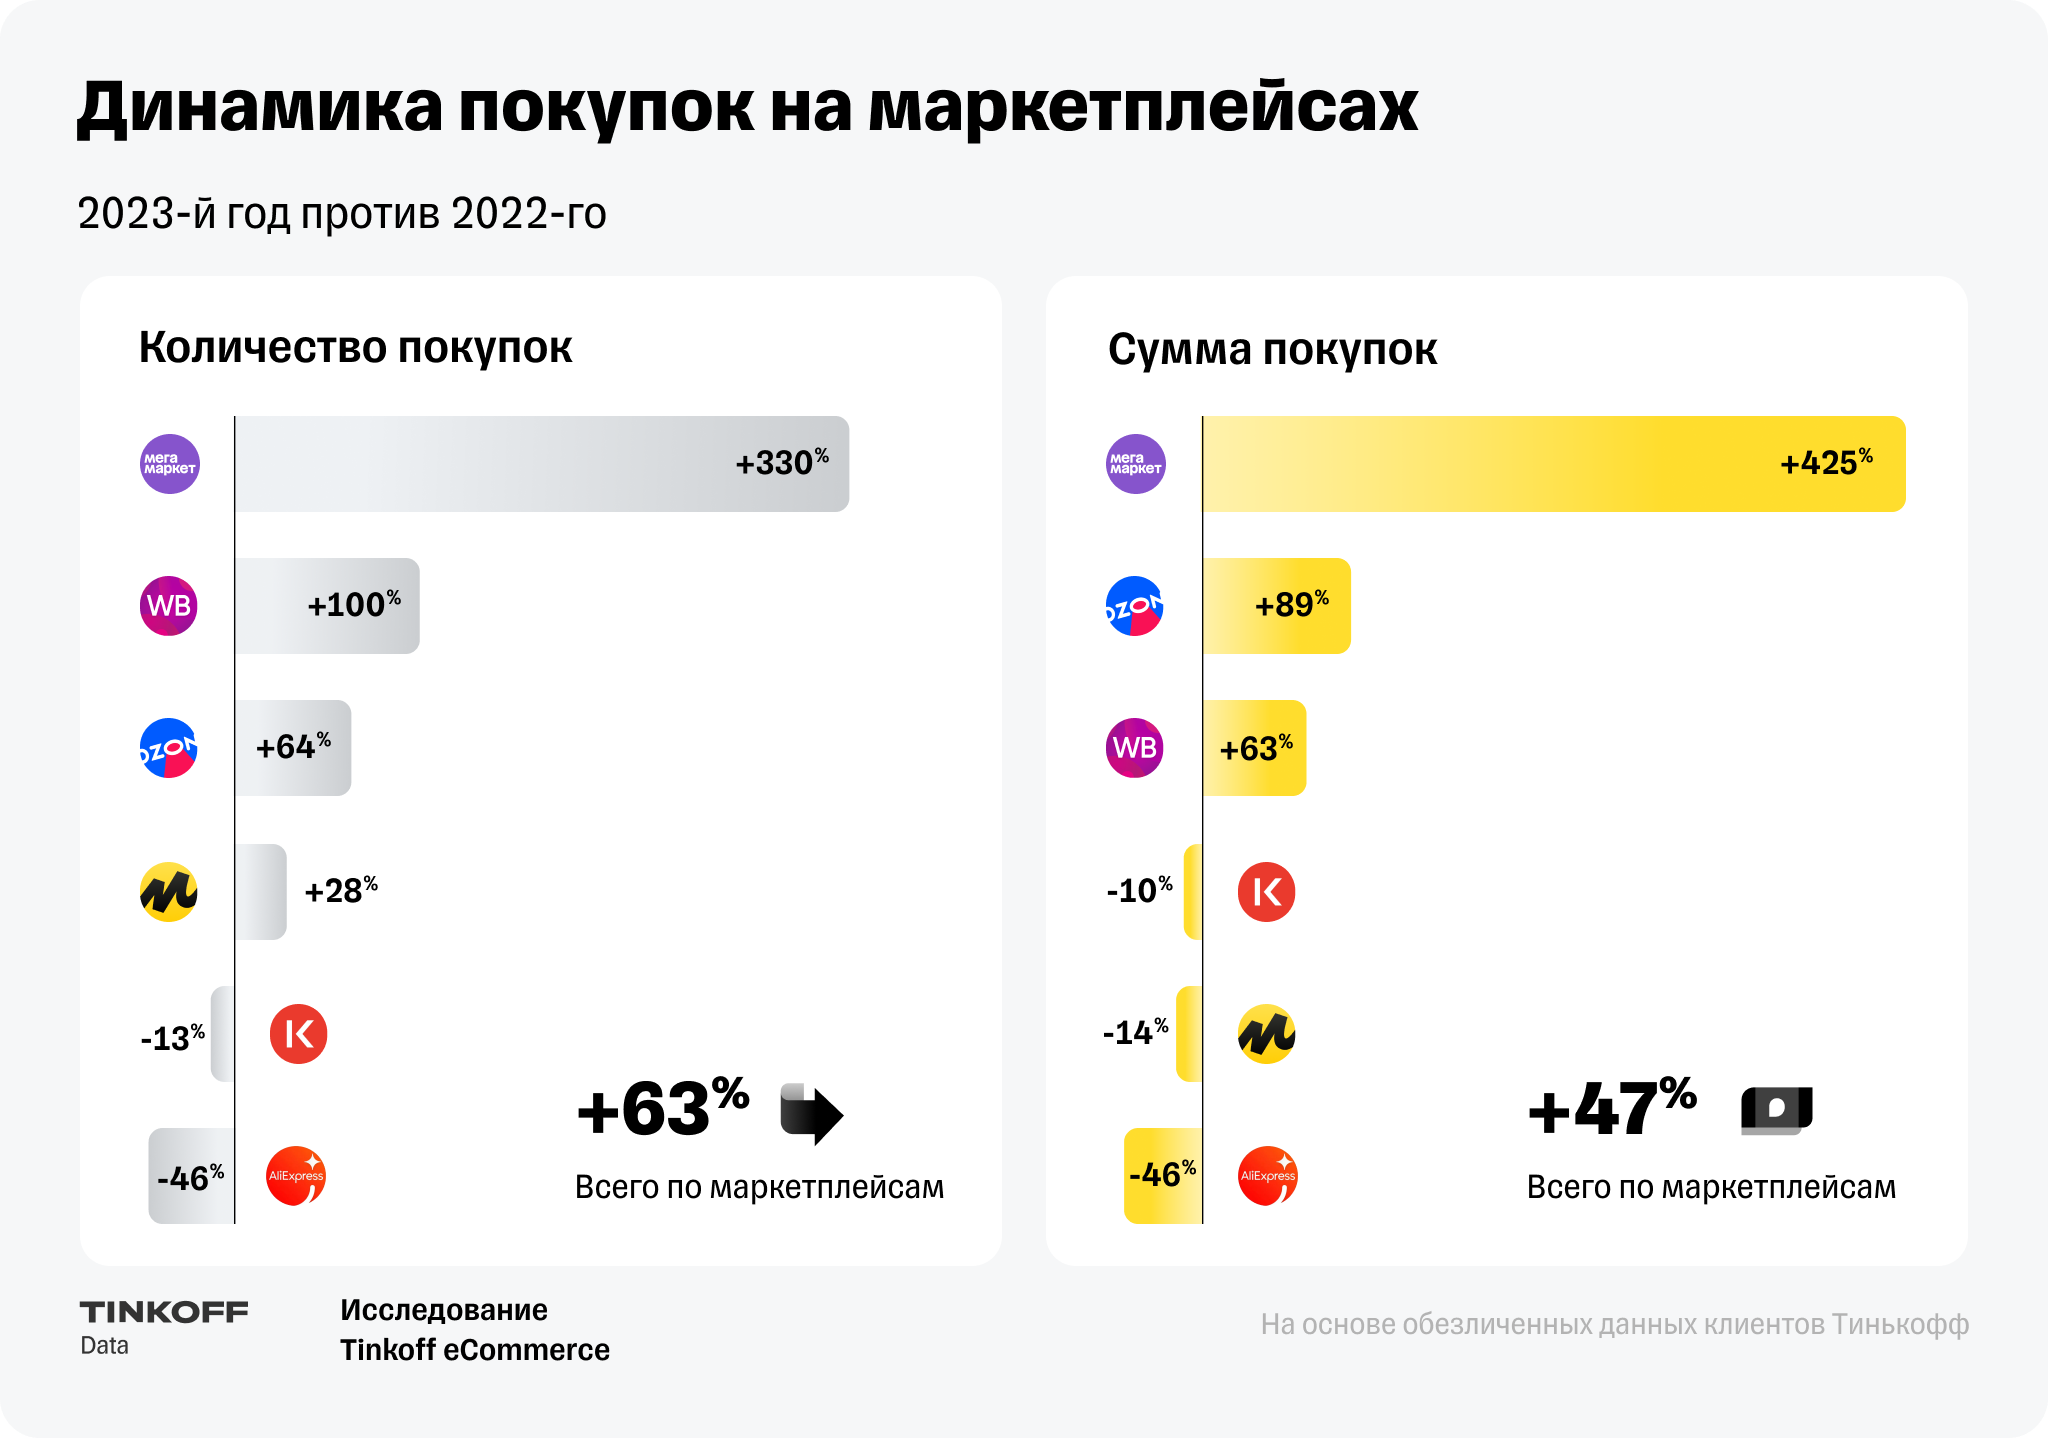
\includegraphics[scale=0.3]{marketplaces-purchases-increased.png}
	\caption{Динамика покупок на маркетплейсах в регионах.}
	\label{fig:marketplaces-purchases-increased}
\end{figure} 

Появился тренд на рост популярности маркетплейсов в российских регионах. В 2023 году жители российских городов стали значительно активнее совершать покупки на маркетплейсах: выросло как количество транзакций на онлайн-площадках, так и их сумма (см. рисунок ~\ref{fig:marketplaces-regions}). По количеству совершенных транзакций особенно заметен рост в таких городах, как Омск (+91\%), Красноярск (+88\%), Новосибирск (+79\%), Челябинск (+79\%) и Волгоград (+75\%). В Москве зафиксирован наименьший прирост числа транзакций (+41\%). Увеличение интереса жителей регионов к маркетплейсам объясняется рядом причин: расширением географии присутствия площадок, развитием сетей ПВЗ и логистических сервисов, улучшением условий доставки.

\begin{figure}[hbtp]
	\centering
	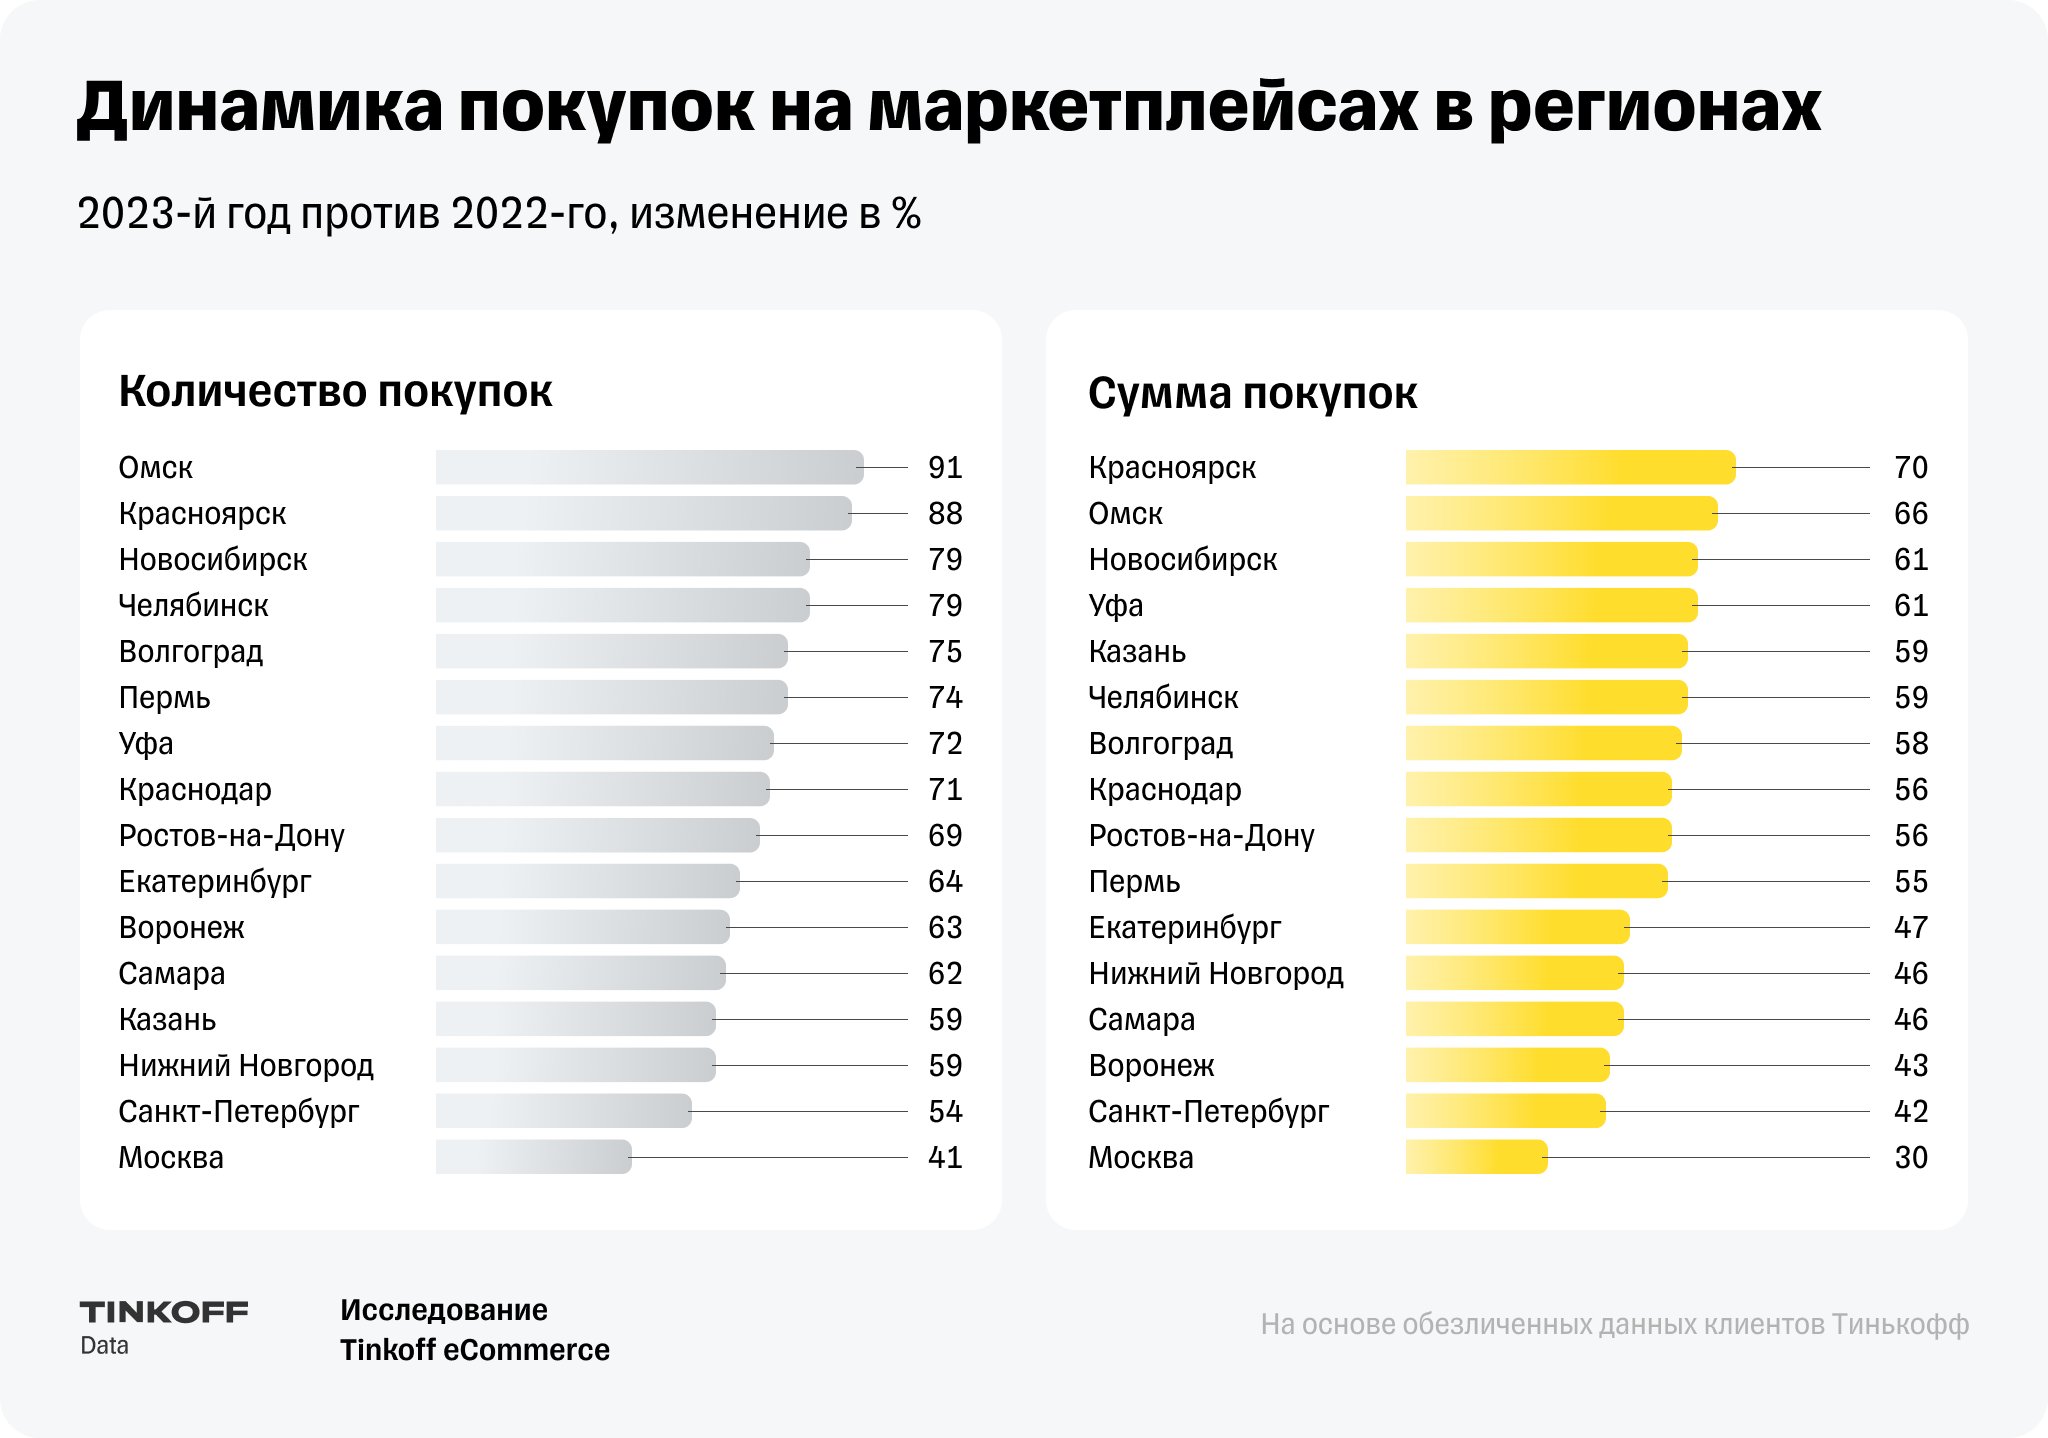
\includegraphics[scale=0.3]{marketplaces-regions.png}
	\caption{Динамика покупок на маркетплейсах в регионах.}
	\label{fig:marketplaces-regions}
\end{figure}  

Вместе с тем выросло количество селлеров на 8\%. Рынок становится более зрелым: место неопытных продавцов занимают более профессиональные. Они ведут бизнес более уверенно, укрепляют свои позиции на площадках и торгуют на нескольких платформах одновременно. Количество селлеров, ведущих торговлю на двух и более маркетплейсах, за год увеличилось на 17\%. Самой привлекательной платформой для старта бизнеса является Wildberries: 63\% продавцов в конце 2023 года выбирали ее в качестве первой площадки (см. рисунок ~\ref{fig:marketplaces-top}).

\begin{figure}[hbtp]
	\centering
	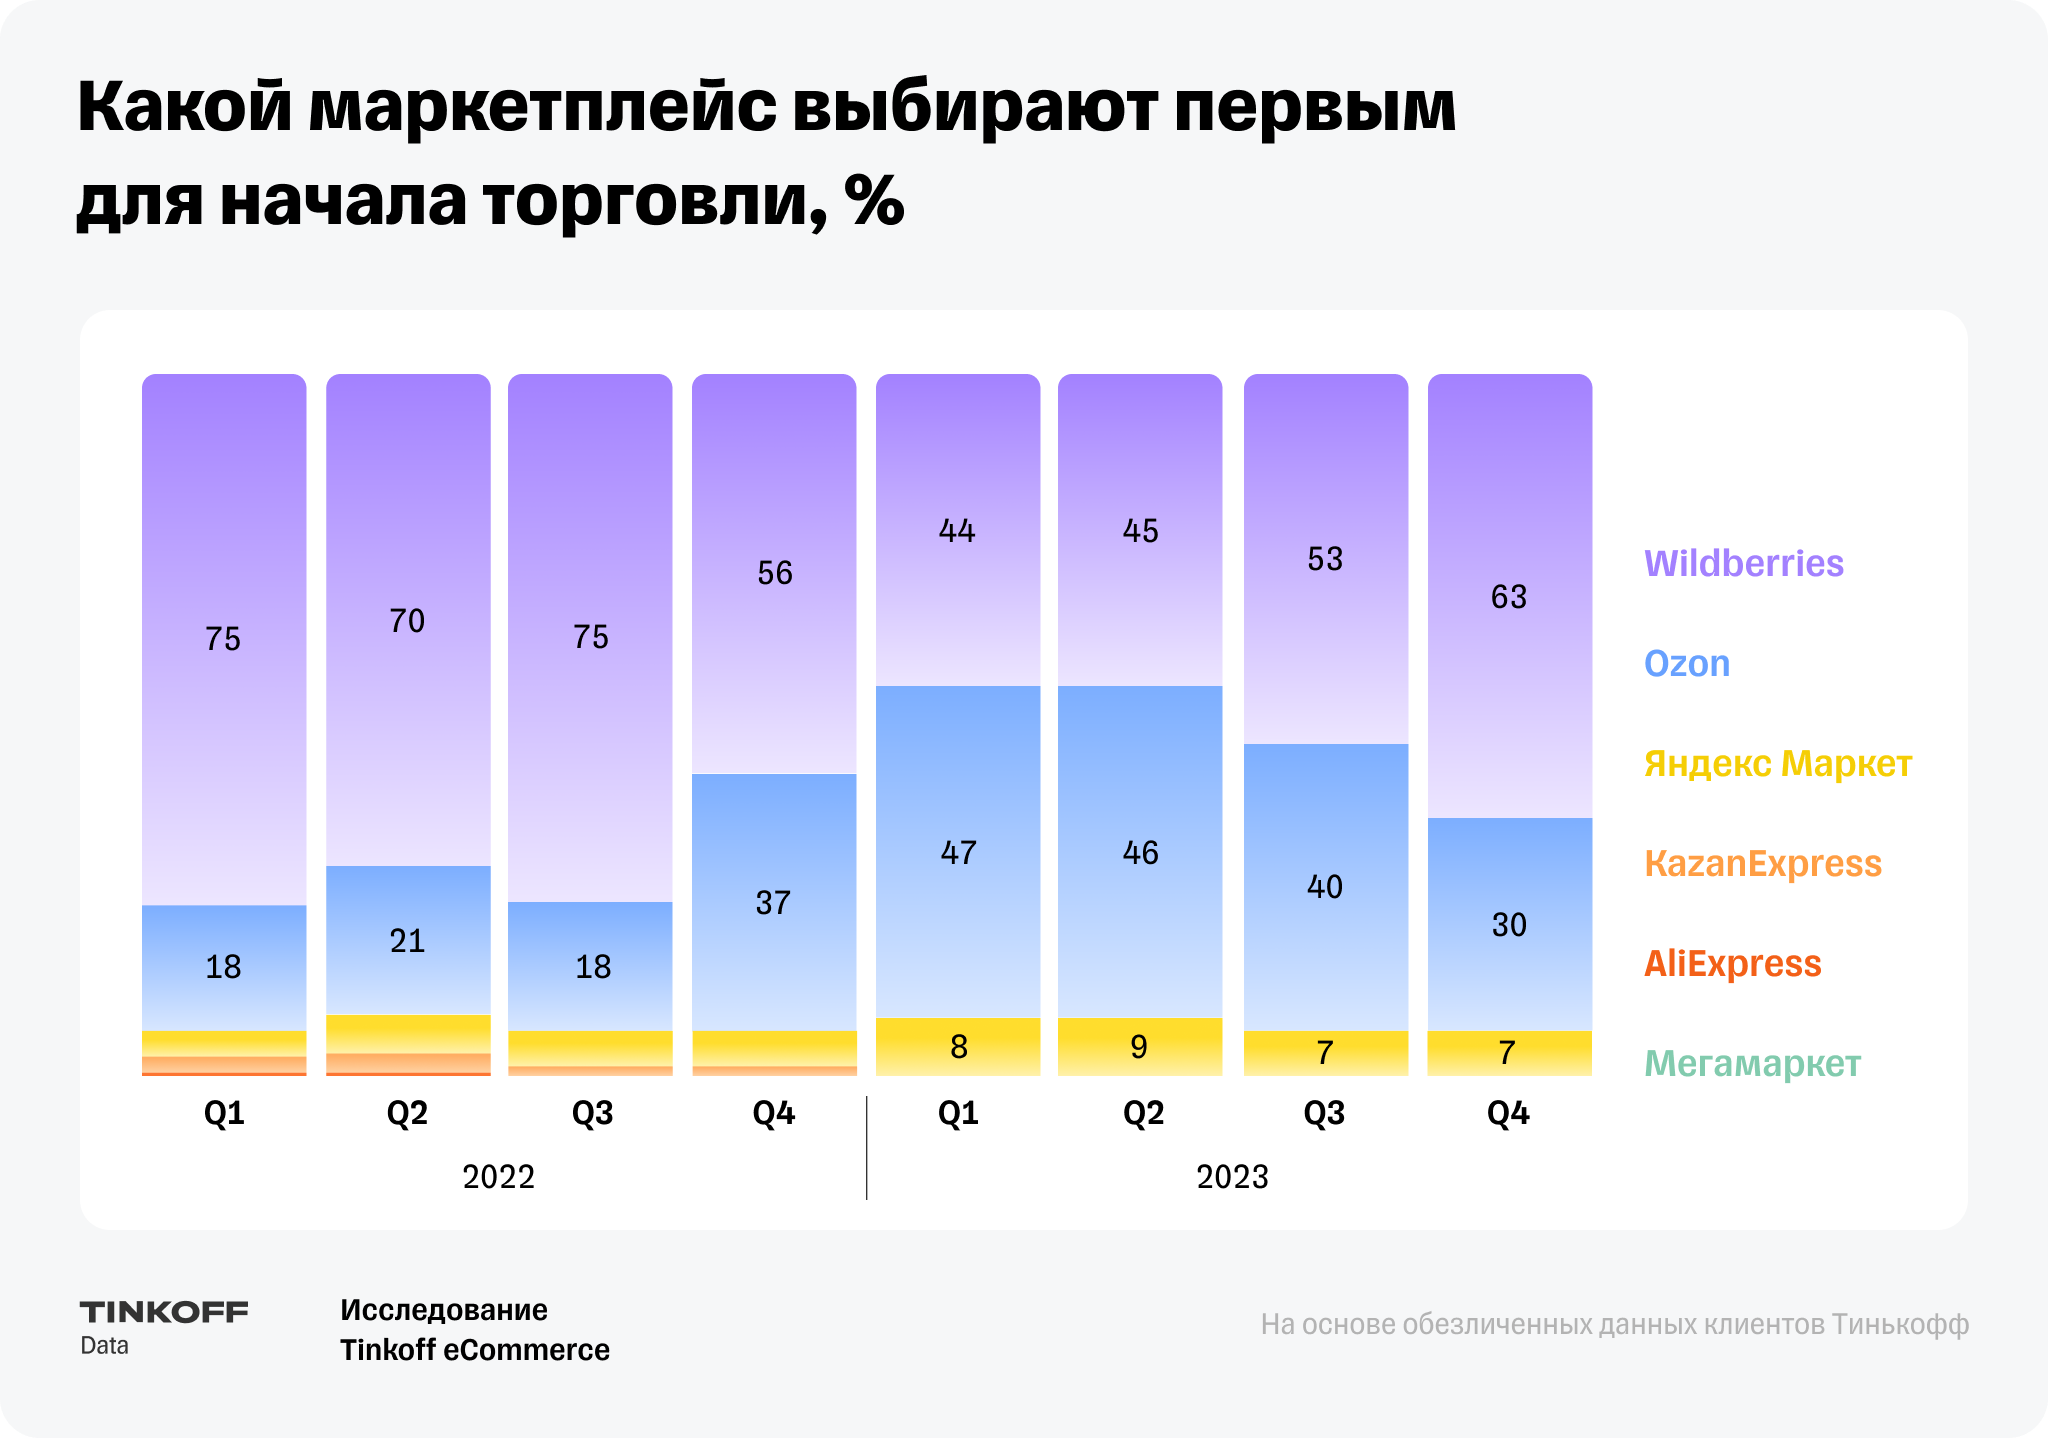
\includegraphics[scale=0.3]{marketplaces-top.png}
	\caption{Популярность маркетплейсов за 2023 год.}
	\label{fig:marketplaces-top}
\end{figure} 

С увеличением конкуренции продавцы все чаще обращаются к системам, которые могут помочь им в продажах, а также автоматизировать процесс работы. Одним из ключевых факторов успешной продажи становится эффективная SEO-оптимизация карточек товаров. Подбор наиболее подходящей категории и создание продаваемого описания, содержащего ключевые слова, позволяет улучшить видимость товаров в результатах поиска как на самом маркетплейсе, так и в поисковых системах, что напрямую влияет на увеличение продаж.

На данный момент существуют несколько сервисов (например, TurboTextPro, CopyMonkey, Gerwin), позволяющих сгенерировать описание товаров по характеристикам, ключевым словам или фото. Однако, качество сгенерированных описаний не всегда позволяют использовать их в системах автономного управления. В настоящее время российский рынок не предлагает специальных технологий и решений для подбора наиболее подходящей категории товара на маркетплейсе. Таким образом, задача создания качественного инструмента для эффективной SEO-оптимизации карточек товаров является актуальной. 

Цель данной работы — разработать сервис, в основе которого будет реализован функционал, способный классифицировать товары на маркетплейсе на основе их фотографий и генерировать соответствующие к ним описания. Сервис реализуется для маркетплейса Wildberries, так как он представляют наибольшую популярность у продавцов и покупателей. В качестве дальнейшего развития проекта можно рассмотреть другие площадки.

Для достижения поставленной цели необходимо решить следующие задачи:
\begin{itemize}
	\item подготовить набор данных, содержащий изображения товаров и соответствующие им категории и текстовые описания;
	\item провести исследование текущих архитектур нейронных сетей, используемых для классификации изображений и генерации текста, и на основе этого исследования выбрать наиболее подходящую архитектуру или их комбинацию для решения поставленной задачи;
	\item обучить выбранную нейронную сеть на подготовленных данных, оптимизировать и настроить параметры модели для повышения её производительности и качества результатов, а затем оценить эффективность реализованной архитектуры нейронной сети;
	\item интегрировать модель в программное обеспечение.
\end{itemize}

\newpage
\section{Данные} 

Данные для поставленной задачи собирались самостоятельно, поскольку в открытых источниках не имелось удовлетворяющего всем требованиям датасета. \textcolor{blue}{(тут можно описать, какие варианты есть).} Как было сказано ранее, выбор маркетплейса пал на «Wildberries». Соответственно данные собирались согласно особенностям структуры данного маркетплейса. Для удобства введем некоторые термины, которыми будем оперировать далее:
\begin{itemize}
	\item \textbf{Карточка товара} – это страница продукта на маркетплейсе, где размещена информация о товаре, фотографии, описание цены и кнопка «Купить»
	\item \textbf{Конечная категория} – это категория, на которых располагаются карточки товаров
	\item \textbf{Материнская категория} – это категория, которая содержит конечные и материнские категории и на которой не располагаются карточки товаров
\end{itemize}

Каталог «Wildberries» разделен на категории, в которых размещены карточки товаров одного типа. Категории выстроены по принципу дерева. Есть основные «широкие» категории, такие как «Женщинам», «Дом», «Продукты», которые объединяют внутри себя более мелкие подкатегории. Например, в разделе «Дом» имеются подкатегории «Ванная», «Кухня», «Спальня» и тд, которые в свою очередь могут подразделяться на еще более маленькие подкатегории. 

Требуемые данные располагались на товарных карточках, в которые можно попасть только зная конечную категорию товара. Поэтому было принято решение разделить сбор данных на 2 этапа. На первом этапе был произведен сбор всех имеющихся на «Wildberries» конечных категорий. На втором – сбор необходимой информации с карточек товаров.

\subsection{Этап 1}

«Wildberries» предлагает 22 основные категории (см. рисунок~\ref{fig:wildberries1}), из которых одна является конечной категорией. Данные категории в дальнейшем будем называть категориями первой вложенности. Их подкатегории, соответственно, будут называться категориями второй вложенности. И так далее, спускаясь все ниже по дереву категорий. Экспериментальным путем была выявлена максимальная глубина вложенности – 5.

\begin{figure}[hbtp]
	\centering
	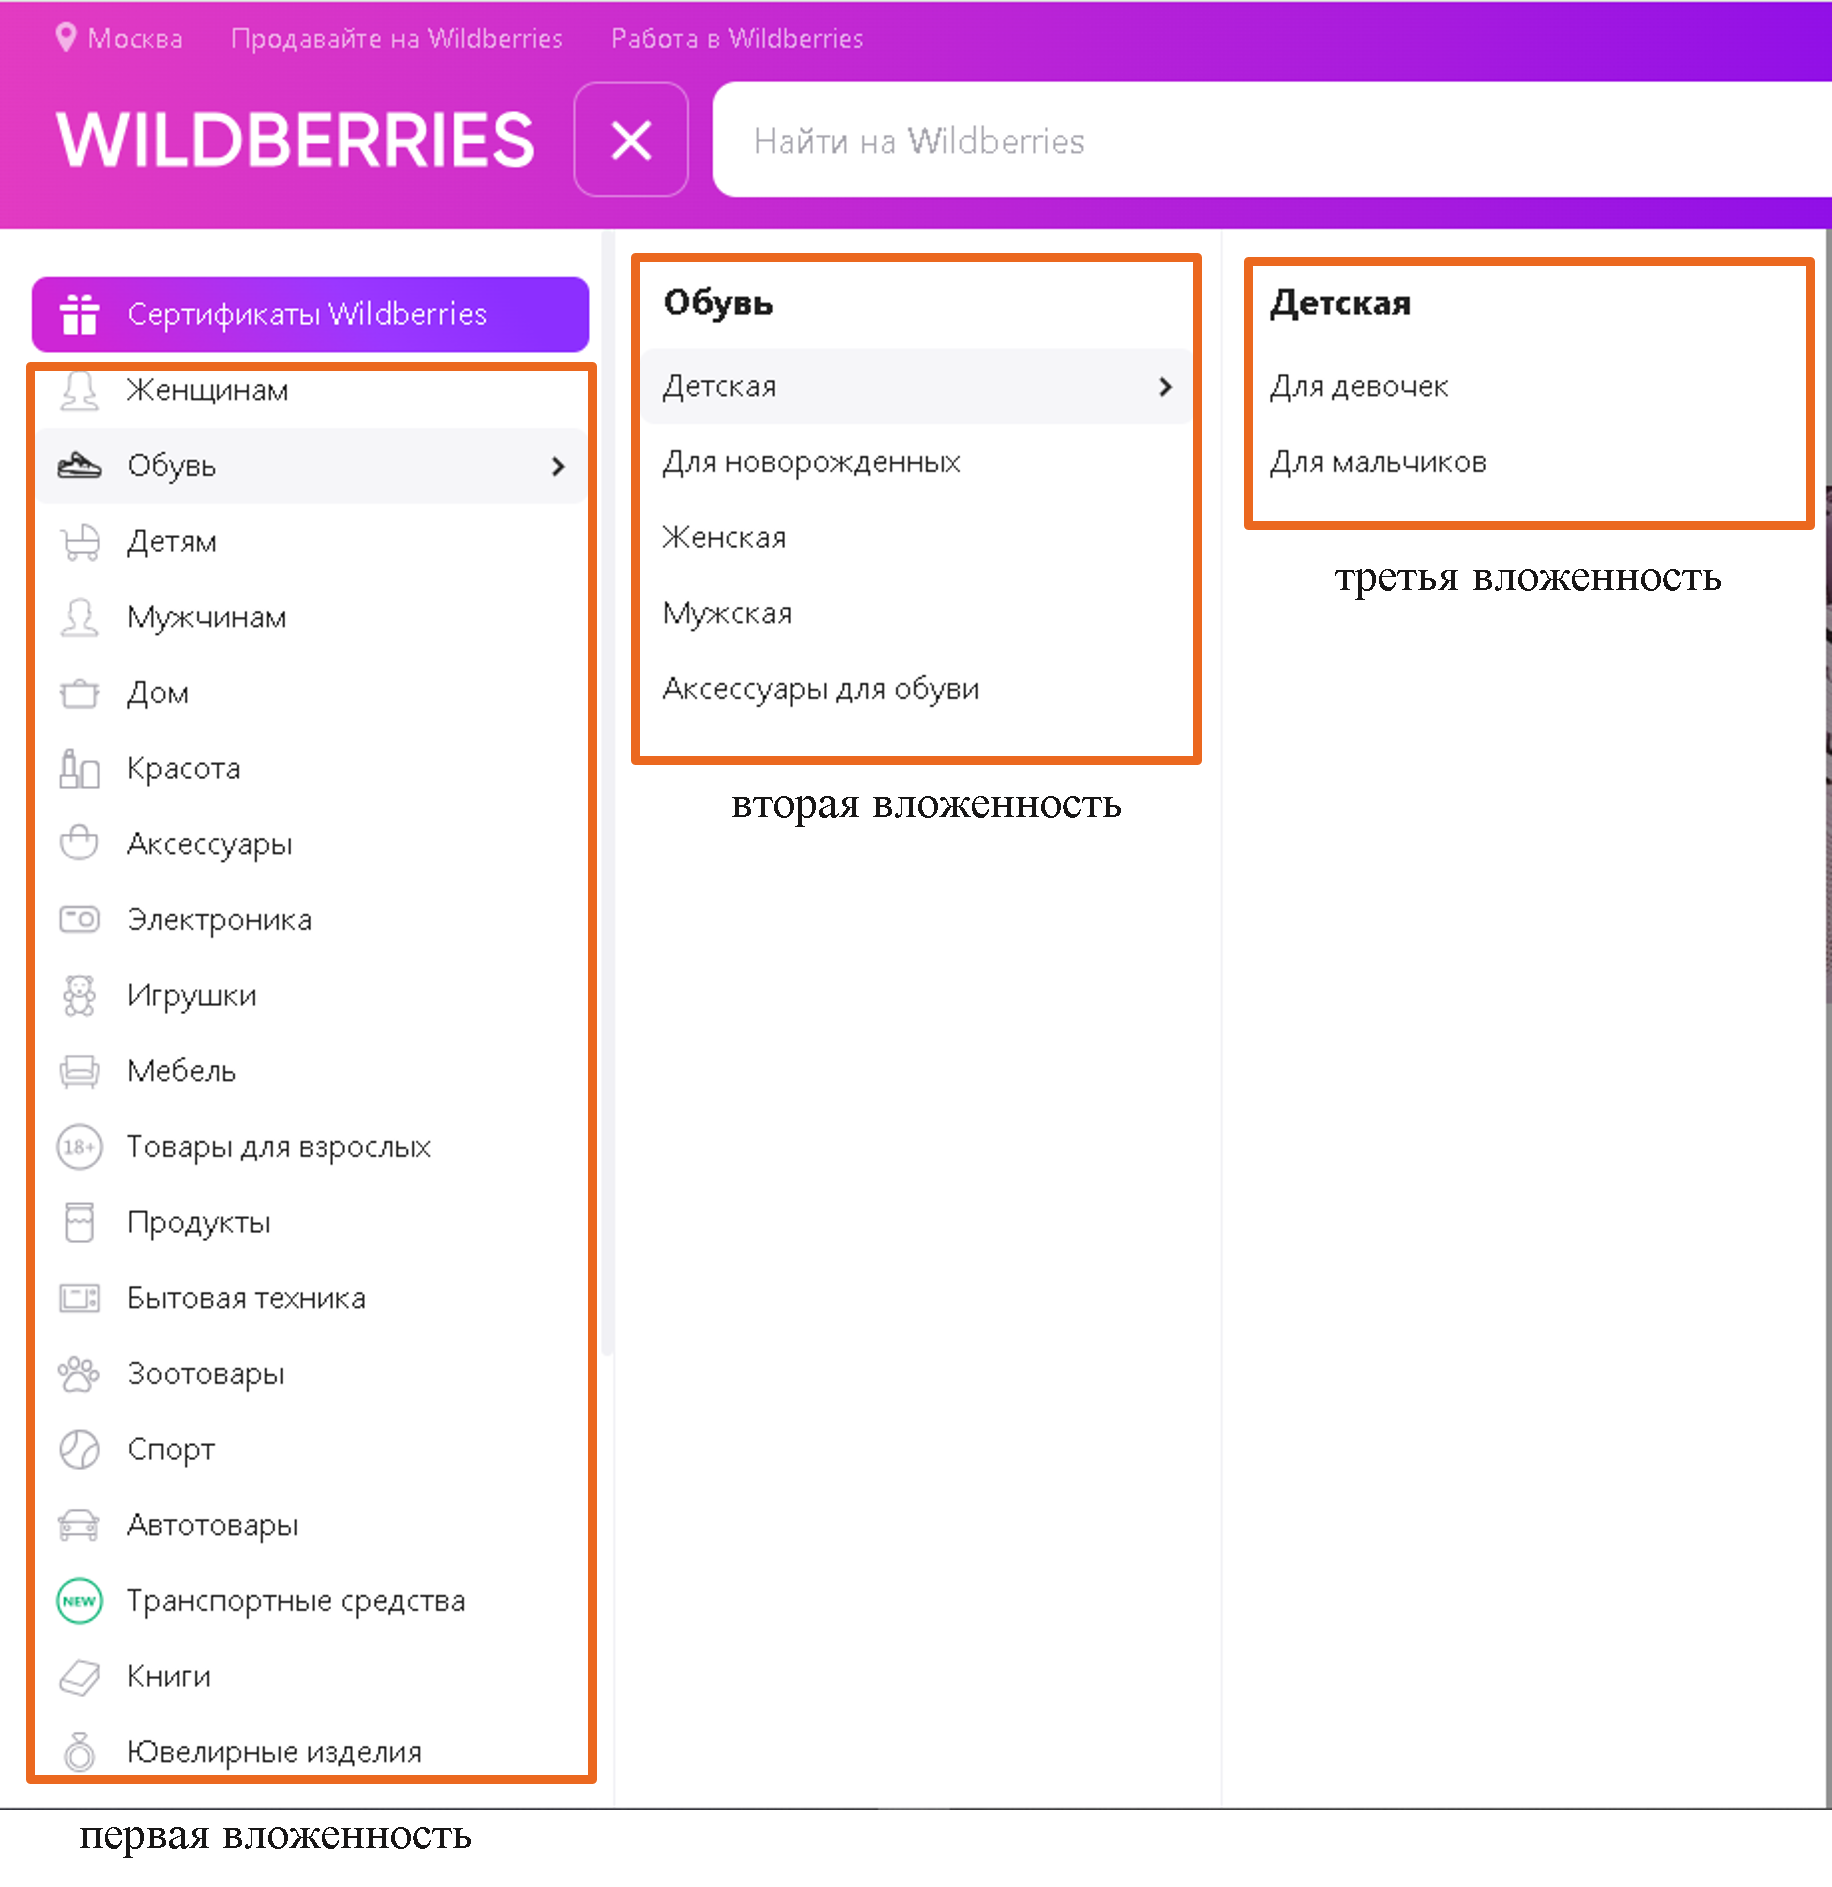
\includegraphics[scale=0.8]{wildberries1.png}
	\caption{Структура каталога «Wildberries» на примере категории «Обувь».}
	\label{fig:wildberries1}
\end{figure} 

Для правильного формирования таргета для классификации при сохранении ссылки на конечную категория нужно было учитывать весь путь по дереву категорий, начиная с первой вложенности. Решением данной задачи стало создание таблицы, где отражалось какие категории было предшествовавшими конкретной конечной категории (см. таблицу~\ref{table:datastatistic0}). При отсутствии более глубокой вложенности на месте данных категорий ставились «NaN». Таким образом, было собрано 1668 конечных категорий.

\begin{table}[ht]
\caption{Фрагмент таблицы, полученной после первого этапа сбора данных.}
\label{table:datastatistic0}
\footnotesize
\centering
	\begin{tabular}{lrrrrrr}
		\toprule
		{} & \multicolumn{1}{c}{$\mathsf{category_1}$} &\multicolumn{1}{c}{$\mathsf{category_2}$} &  \multicolumn{1}{c}{$\mathsf{category_3}$} & \multicolumn{1}{c}{$\mathsf{category_4}$} &  \multicolumn{1}{c}{$\mathsf{category_5}$} & \multicolumn{1}{c}{$\mathsf{url}$}\\
		\midrule
		437 & Дом & Предметы интерьера & Фоторамки и фотоальбомы & Фотоальбомы       & NaN              & https://www.wildberries.ru/catalog/dlya-doma/predmety-interera/fotoramki-i-fotoalbomy/fotoalbomy\\
		438 & Дом & Предметы интерьера & Картины и постеры       & Рамы для постеров & NaN              & https://www.wildberries.ru/catalog/dlya-doma/predmety-interera/kartiny/ramy-dlya-posterov\\
		439 & Дом & Предметы интерьера & Картины и постеры       & Постеры           & Детская тематика & https://www.wildberries.ru/catalog/dlya-doma/predmety-interera/kartiny/postery/detskaya-tematika\\
		440 & Дом & Предметы интерьера & Картины и постеры       & Картины           & Арт и абстракция & https://www.wildberries.ru/catalog/dlya-doma/predmety-interera/kartiny/kartiny/art-i-abstraktsiya\\
		441 & Дом & Предметы интерьера & Картины и постеры       & Постеры           & Фэнтези          & https://www.wildberries.ru/catalog/dlya-doma/predmety-interera/kartiny/postery/fentezi\\
		\bottomrule
	\end{tabular}
\end{table}

Составление данной таблицы производилось посредством парсинга данных с сайта «Wildberries» через Python с использованием библиотек selenium и BeautifulSoup. Блокировок со стороны маркетплейса замечено не было. Особенность и неудобством парсинга была динамическая подгрузка страниц, которая вынуждала выдерживать паузы в несколько секунд для удовлетворяющей прогрузке страницы. Данное обстоятельство привело с значительному увеличению времени парсинга данных.

При анализе собранной таблицы были выявлены некоторые особенности категориальной политики «Wildberries». Во-первых, категории у данного маркетплейса не фиксированы. Например, было отмечено, что часть категорий активно перемещается из раздела в раздел, какие-то категории могут пропадать, также могут появляться новые категории. Данные, собранные в текущем датасете, актуальны на конец января 2024 года. Однако для поддержания списка категорий в актуальном состоянии необходимы механизмы регулярного обновления данных. Во-вторых, на маркетплейсе имеются конечные категории, ссылающиеся на одни и те же url страницы. Подобные категории будут называться дублирующими. Подобные дубляжи могли иметь разное происхождение: особенности маркетинга и неудачное время парсинга, выпавшее на перемещение категорий. С точки зрения маркетинга подобные дублирования оправданы, поскольку потенциальный покупатели могут по своим соображениям относить одни и те же товары к разным категориям. Для примера, категория «Коврики» находилась в разделе «Автотовары\_Коврики» и «Электроника\_Автоэлектроника\&и\&навигация\_Коврики». Для корректной работы модели была написана отдельная процедура удаления подобных дублирующих категорий. Выбор, какой из дубликатов оставлять, производился вручную. Всего было найдено 69 дублирующих ссылок, которые могли встречаться 2 и более раза. Таким образом, после удаления в таблице осталось 1580 категорий.

Далее можно было переходить ко 2му этапу.


\subsection{Этап 2}

Второй этап сбора данных заключался в прохождении по собранному ранее списку конечных категорий и сбора из каждой из них информации с карточек товаров. Было принято решение брать по 20 товаров из каждой конечной категории. Из каждой карточки товара сохранялось первое фотография от продавца, первая фотография из отзыва и описание товара (см. рисунок~\ref{fig:wildberries2}). Первая фотография от продавца бралась по причине ее обязательного присутствия в карточке товара, а также гарантированного качественного изображения товара на ней. Однако поскольку разрабатываемый сервис рассчитан на работу в большинстве случаев с фотографиями от пользователей, все дефекты, присущие любительским фотографиям могут иметь место быть. Поэтому для стабильности предсказаний классификационной модели, было решено подавать в нее также фотографии из отзывов, которые максимально близко будут похожи на фотографии, с которыми будет работать в дальнейшем сервис. Описания товара были нужны для задачи генерации текстовых описаний к изображениям. В итоге при полном наборе для каждой конечной категории имелось 40 фотографий (20 фотографий от продавцов и 20 фотографий из отзывов) и 20 описаний.

\begin{figure}[hbtp]
	\centering
	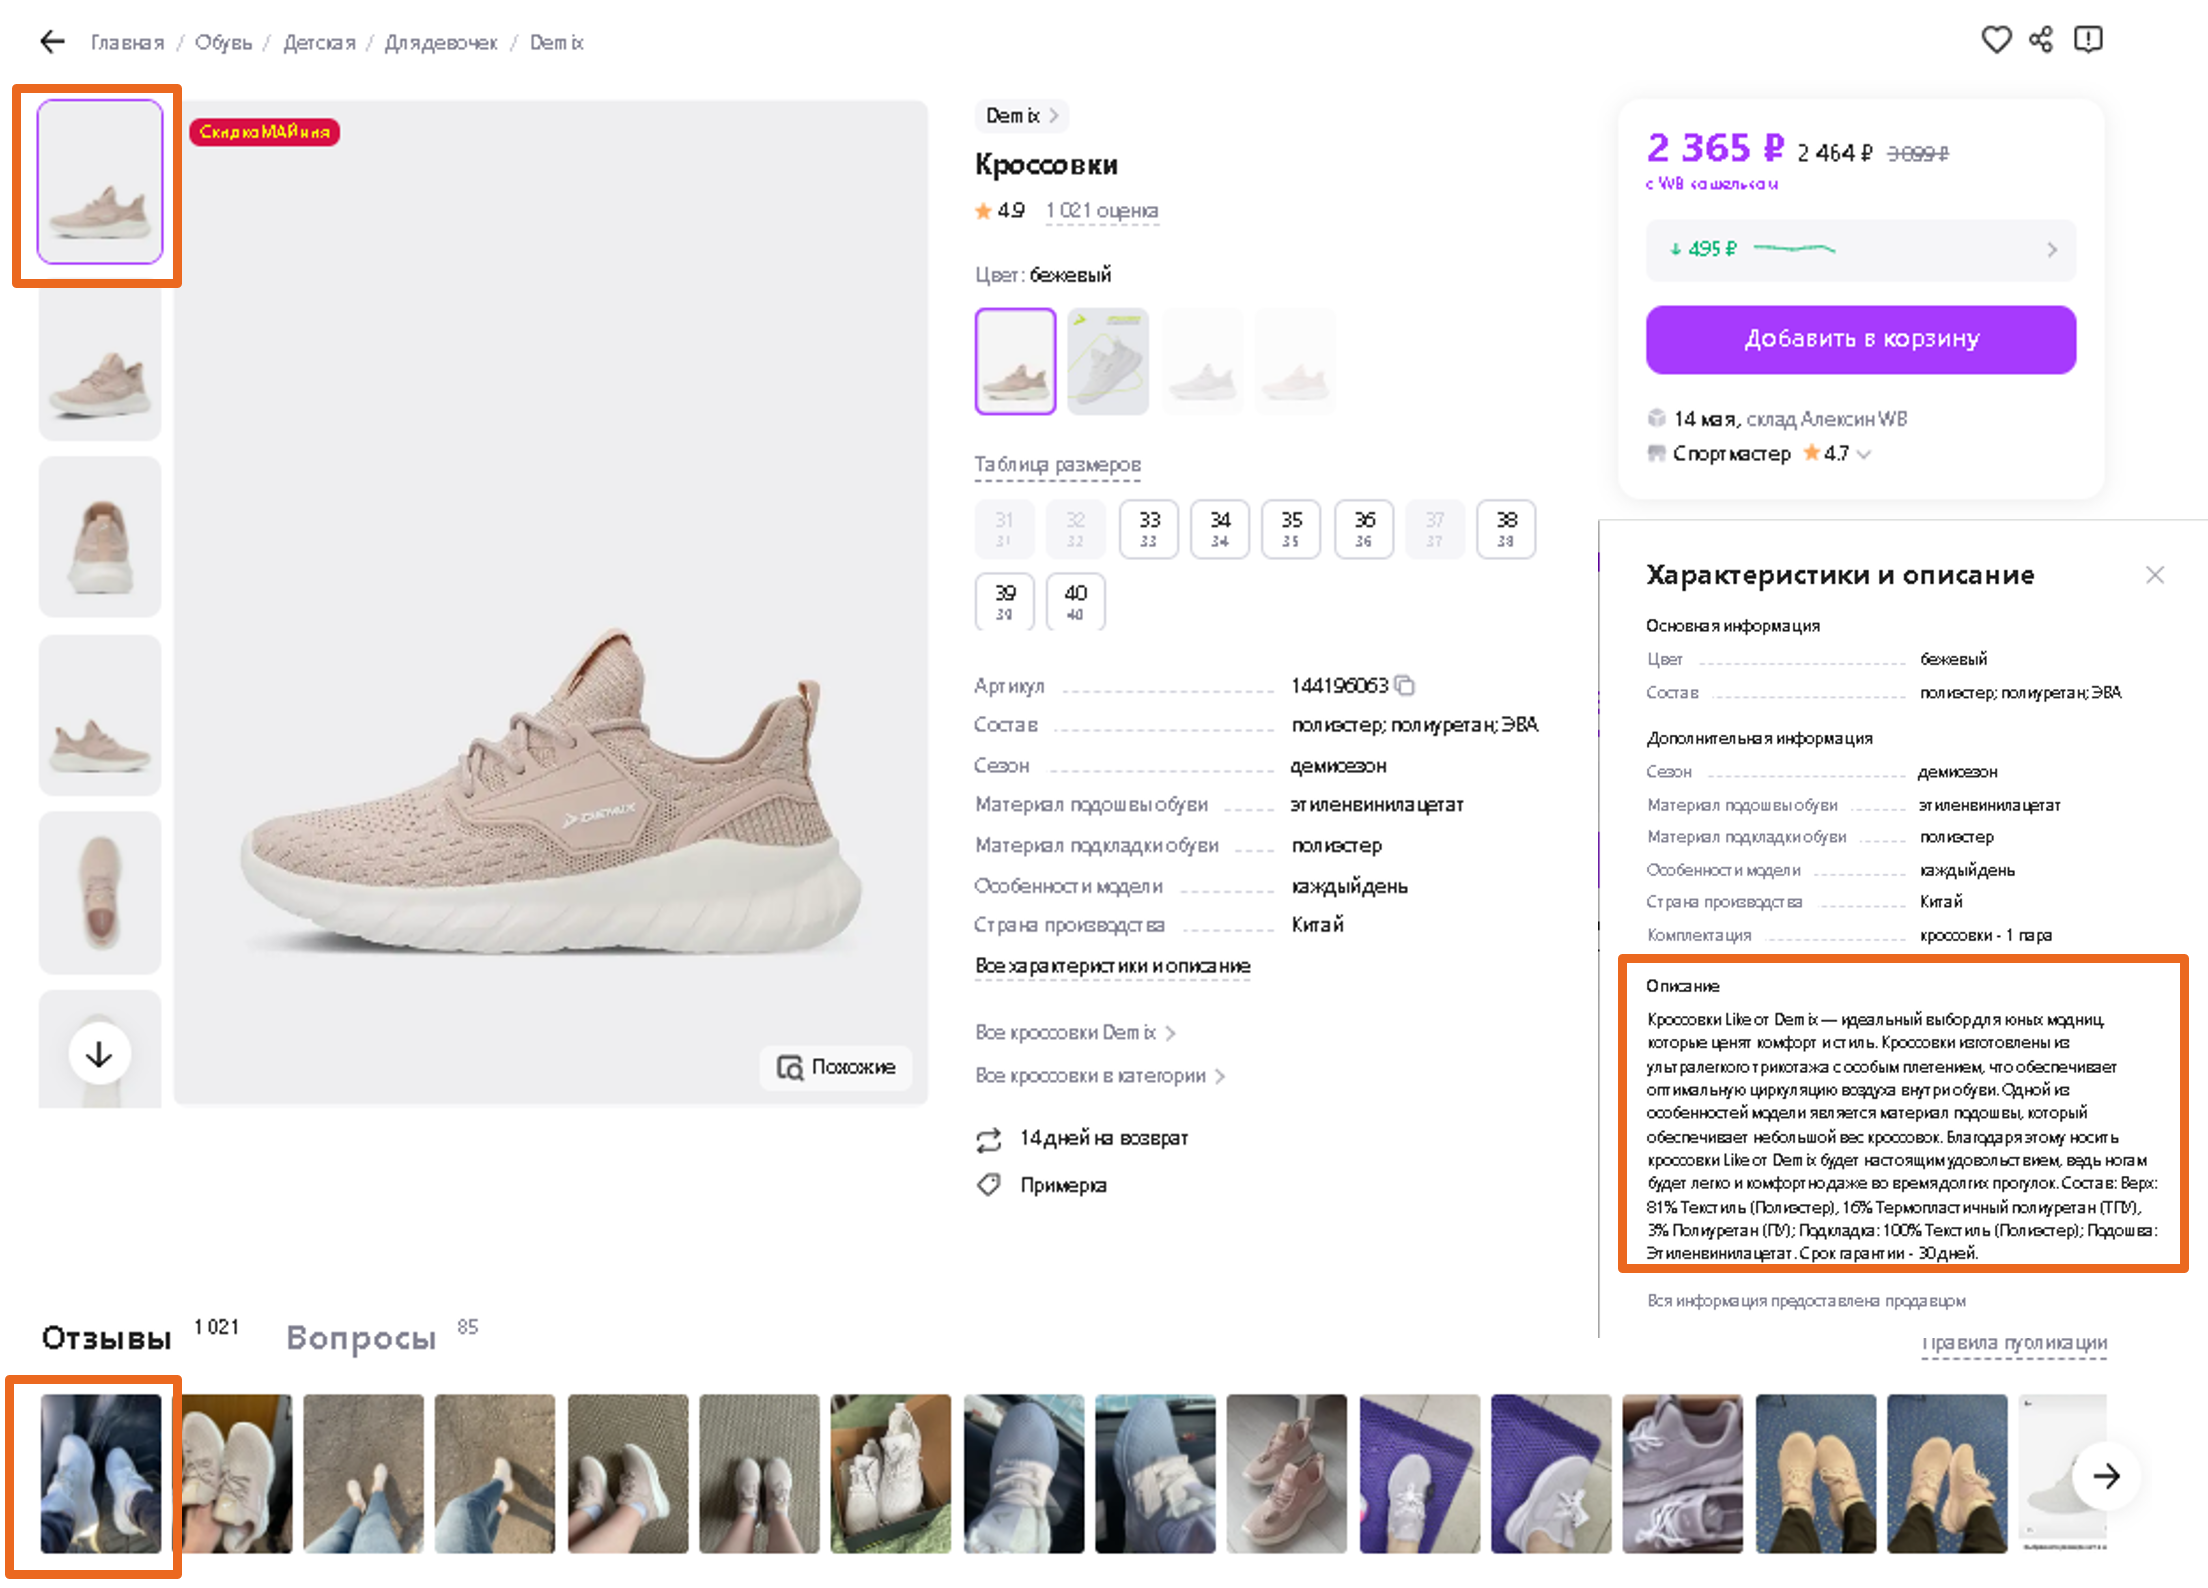
\includegraphics[scale=0.8]{wildberries2.png}
	\caption{Пример карточки товара на «Wildberries». Верхний левый прямоугольник – первая фотография от продавца. Нижний левый прямоугольник – первая фотография из отзыва. Правый прямоугольник – текстовое описания товара.}
	\label{fig:wildberries2}
\end{figure}

При выполнении данного этапа было несколько трудностей. Во-первых, стандартная на «Wildberries» динамическая прогрузка страниц, увеличивающая время парсинга более чем в 3 раза. Приходилось делать паузы при открытии страницы с карточкой товара, при открытии описания, лежащее в отдельной вкладке, и пролистывание страницы вниз для подгрузки информации об отзывах. Примерное время парсинга данных, затраченное на второй этап, равнялось 2м неделям. Во-вторых, имели товары с меткой «18+», для которых требовалось дополнительное нажатие кнопки, подтверждающее достижение указанного возраста. В-третьих, некоторые поля в карточке товара заключали в себе картинки, которые вынуждали в определенных случаях дополнительно пролистывать страницу вниз. В-четвертых, для нажатия кнопки с целью получения описание к товару, выдвигалось требование расположение кнопки в зоне видимости экрана. Это приводило к еще более тонкой настройке пролистывания страницы, подобранной под конкретный размер экрана компьютера.

Для сохранения данных из карточек товара была придумала специальная структура с целью дальнейшего удобства использовании в задаче классификации и генерации текста. Все товары, собранные из одной конечной категории, сохранялись в отдельную папку, содержащую следующие элементы:
\begin{itemize}
	\item папку «card», куда складывались фотографии от продавцов
	\item папку «feedbacks», куда складывались фотографии из отзывов
	\item файл «descriptions.csv», где сохранялись описания к товарам
\end{itemize}

Название данной папки определялось посредство таблицы 1 и складывалось из всех материнских категорий, участвовавших в пути к конечной категории. Например, для конечной категории «Фотоальбомы» (см. таблицу~\ref{table:datastatistic0}) название папки было следующее: «Дом\_Предметы\&интерьера\_Фоторамки\&и\&фотоальбомы\_Фотоальбомы», а для категории «Фэнтези» - «Дом\_Предметы\&интерьера\_Картины\&и\&постеры\_Постеры\_Фэнтези». Более подробно об использовании подобной структуры ранения данных будет описание в главе \_\_\_ в разделе \_\_\_.

Первичный анализ собранных данных выявил, что не у всех товаров имелись отзывы с фотографиями и описания. Описания имелись в 99.8\% проценте случаев. В таблице~\ref{table:datastatistic1} приведены некоторые статистические данные о собранных фотография от продавца и из отзыва. Можно заметить, что некоторые конечные категории были полностью без фотографий в отзывах. Однако, опираясь на перцентили, можно сделать вывод, что таких категорий было довольно мало. Касательно фотографий от продавцов можно сделать 2 вывода. Во-первых, есть категории, представленные менее чем 20ю товарами. Во-вторых, есть как минимум одна категория, в которой имеется только 1 товар. Подобные категории нас не устраивают, потому что далее будет производиться деление каждой категории на 2 части, и категории с одним товаром невозможно будет разделить.

\begin{table}[ht]
	\caption{Описательная статистика по фотографиям от продавца (столбец «card») и фотографиям из отзыва (столбец «feedbacks»).}
	\label{table:datastatistic1}
	\footnotesize
	\centering
	\begin{tabular}{l|rr}
		\toprule
		{} & \multicolumn{1}{c}{$\mathsf{card}$} & \multicolumn{1}{c}{$\mathsf{feedbacks}$}\\
		\midrule
		count &	1580  & 1580\\
		mean  & 19.98 & 17.72\\
		std   & 0.63  &	4.23\\
		min   &	1     &	0\\
		25\%  &	20    &	18\\
		50\%  &	20    &	19\\
		75\%  &	20    &	20\\
		max   &	20    &	20\\
		\bottomrule
	\end{tabular}
\end{table}

Всего категорий, представленных менее 20 товарами, было выявлено 5 штук (см. таблицу~\ref{table:datastatistic2}). Из них представляли наибольший интерес \_ и \_, из-за чересчур малого количества товаров. Категорию с одним товаром было решено удалить. Таким образом, осталось 1579 конечных категорий, с которыми шла вся дальнейшая работа.

\begin{table}[ht]
	\caption{Таблица с категориями, имеющими менее 20 товаров.}
	\label{table:datastatistic2}
	\footnotesize
	\centering
	\begin{tabular}{rc}
		\toprule
		\multicolumn{1}{c}{кол-во товаров} & \multicolumn{1}{c}{категория}\\
		\midrule
		18 & Дом\_Кухня\_Кухонный\&текстиль\_Чехлы\&для\&ручек\&холодильников\\
		4  & Дом\_Освещение\_Лифты\&для\&люстр\\
		19 & Мебель\_Гардеробная\&мебель\_Ящики\\
		1  & Мебель\_Офисная\&мебель\_Перегородки\&офисные\\
		19 & Мебель\_Офисная\&мебель\_Шкафы\\
		\bottomrule
	\end{tabular}
\end{table}

При более детально рассмотрении собранных данных было замечено, что фотографии из отзывов довольно шумные (см. рисунок~\ref{fig:dataexample1}). Очень много одинаковых фотографий, фотографий, где не очень понятно, что изображено. Поэтому для дальнейшей работы использовались только фотографии товара от продавца.

\begin{figure}[hbtp]
	\centering
	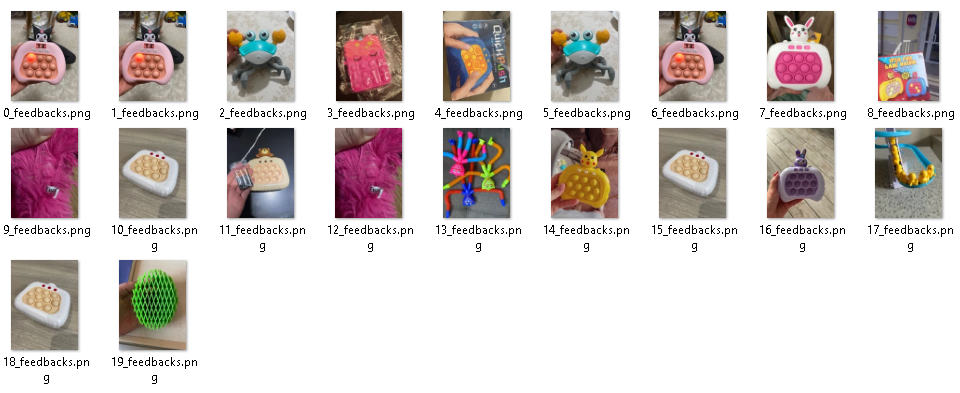
\includegraphics[scale=0.8]{dataexample1.png}
	\caption{Фотографии из отзывов в категории «Игрушки\_Антистресс».}
	\label{fig:dataexample1}
\end{figure}

Далее интересно было рассмотреть количество собранных данных в разрезе категорий первой вложенности (см. рисунок~\ref{fig:amount_of_categoty}). Из круговой диаграммы можно заметить, что категории довольно несбалансированный. Например, категория «Дом» вмещает в себя порядка 6000 пример. В то время как в категории «Ювелирные\&изделия» только 320 примеров.

\begin{figure}[ht]
	\centering
	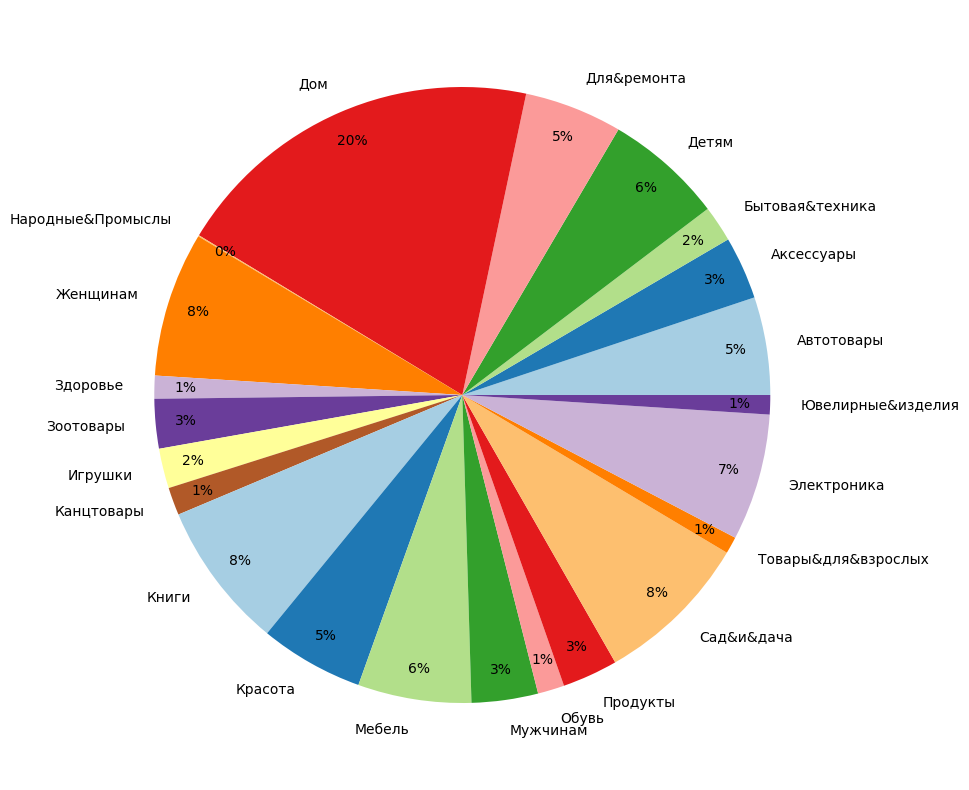
\includegraphics[scale=0.8]{amount_of_categoty.png}
	\caption{Распределение данных по категориям первой вложенности.}
	\label{fig:amount_of_categoty}
\end{figure}

Подобную картину можно наблюдать в категориях всех вложенностей (см. приложение~\ref{appendix:amount_of_categor2}).

После появление базового понимания данных надо было приступать к их детальному изучению. Как правило, парсинг большого количества данных, тем более с постоянно меняющихся маркетплейсов, не проходит идеально. В сохраненных данных могут быть оплошности, которые помешают грамотно решать задачу классификации и генерации текста. Приведем некоторые примеры, выявленных особенностей, требуемых принятие решений с нашей стороны:
\begin{itemize}
	\item Встречаются категории, которые с точки зрения категорийного менеджмента, имеют место быть. Одна для классификационной модели машинного обучения такие категории будут не осиливаемыми. Например, в разделе «Женщинам» есть подкатегории «Женщинам\_Белье» и «Женщинам\_Большие\&размеры\_Белье». Если детально изучить фотографии, которые в этих категориях присутствуют, можно сделать вывод, что особых различий между ними нет. Единственное, что было подмечено, что на очень немногих фотографиях стоит надпись «4XL» или что-то подобное, указывающее, что у данного товара имеются большие размера. Более того, в обеих категориях присутствуют одинаковые товары.
	\item В данных попадались «мусорные» категории. Предположительно, подобное возникало из-за изменения url ссылок на категории со стороны «Wildberries». В подобных категориях находились товары, собранные случайным образом из всевозможных категорий с маркетплейса.
	\item Распределение товаров по категориям не очень четкая задача. В связи с этим встречались одинаковые товары, находящиеся в разных категориях. Например, одна и та же продукт мог находиться в категориях «Зоотовары\_Груминг\&и\&уход», «Зоотовары\_Для\&кошек\_Груминг\&и\&уход» и «Зоотовары\_Для\&собак\_Груминг\&и\&уход».
	\item В части материнских категорий встречались разделы «Подарки» (например, материнские категории «Мужчинам\_Подарки\&мужчинам» и «Женщинам\_Подарки\&женщинам»), куда были собраны товары из совершенно разных категорий, таких как «Аксессуары», «Дом», «Продукты» и тд.
	\item Поскольку при парсинге из каждой категории брались первые 20 товаров, появляется неконтролируемый фактор того, какие товары стоят вначале. Как правило, пользователи смотрят только на первые товары в выдаче. Поэтому на маркетплейсах существуют множество механизмов и правил отбора товаров, которые будут показаны пользователю в начале. В нашем случае было замечено, что некоторые категории стали более шумными из-за сезонных товаров. Например, в категории «Зоотовары\_Фермерство» были найдены пасхальные яйца.
	\item Бывали категории, которые по смыслу имели место быть как отдельные категории, однако в них были собраны не совсем подходящие товары. Например, в категории «Мужчинам\_Религиозная\_Православие» находились обычные рубашки и штаны, часть из которых присутствовала также в категории «Мужчинам\_Рубашки» и «Мужчинам\_Брюки».
\end{itemize}

Приведенные особенности сохраненных данных требовали ручной очистки датасета. Необходимо было применять следующие действия: полное удаление категории, удаление конкретной фотографии из отзыва, удаление товара полностью (фотографию от продавца, из отзыва и описание к нему) и произведение полного переноса товара (фотографию от продавца, из отзыва и описание к нему) из одной категории в другую. Для удобства и быстроты данной процедуры были написаны функции, позволяющие механизмами Python вносить изменения в собранные данные.

По окончании данной процедуры было подмечено, что категории требовали очистки в разной степени. Какие-то категории, как «Зоотовары», требовали практически полного переформирования. Другие категории обходились легкой очисткой, например «Продукты». Некоторые категории совсем не требовала вмешательства. Таким образом, финальный датасет стал состоять из 1459 конечных категорий (см. таблицу~\ref{table:datastatistic2}).

\begin{table}[ht]
	\caption{Описательная статистика по фотографиям от продавца после очистки собранных данных. \textsl{Примечание:} статистика по фотографиям из отзывов не приведена, поскольку, как упоминалось ранее, решено было в дальнейшем работать только с фотографиями от продавца.}
	\label{table:datastatistic3}
	\footnotesize
	\centering
	\begin{tabular}{l|r}
		\toprule
		{} & \multicolumn{1}{c}{$\mathsf{card}$}\\
		\midrule
		count &	1459\\
		mean  & 20.09\\
		std   & 2.32\\
		min   &	4\\
		25\%  &	20\\
		50\%  &	20\\
		75\%  &	20\\
		max   &	54 \\
		\bottomrule
	\end{tabular}
\end{table}

\newpage
\section{Декомпозиция задачи} 

Для достижения целей и задач проекта требуется решить задачу создания подписей к изображениям (англ. image captioning, см. примеры на рисунке ~\ref{fig:image-captioning-example}). Для успешной реализации этой задачи необходимо выбрать подходящие модели и определить метрики, которые будут использоваться для оценки их эффективности.

\begin{figure}[ht]
	\centering
	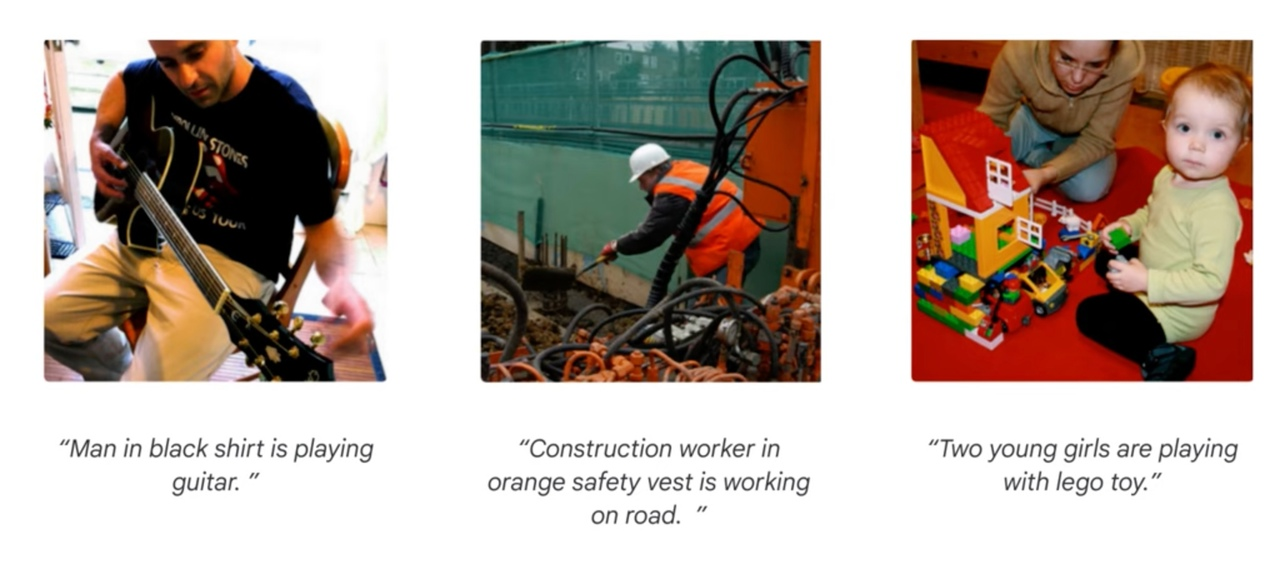
\includegraphics[scale=0.35]{image-captioning-example.png}
	\caption{Примеры задачи Image Captioning.}
	\label{fig:image-captioning-example}
\end{figure}

\subsection{Задача Image Captioning}

Image Captioning — задача создания текстового описания входного изображения, основанная на комбинации сверточных нейронных сетей для обработки изображения и рекуррентных нейронных сетей для генерации подписи, то есть реализующая архитектуру кодировщик-декодировщик (англ. encoder-decoder, см. рисунок ~\ref{fig:image-captioning-arch}).

\begin{figure}[ht]
	\centering
	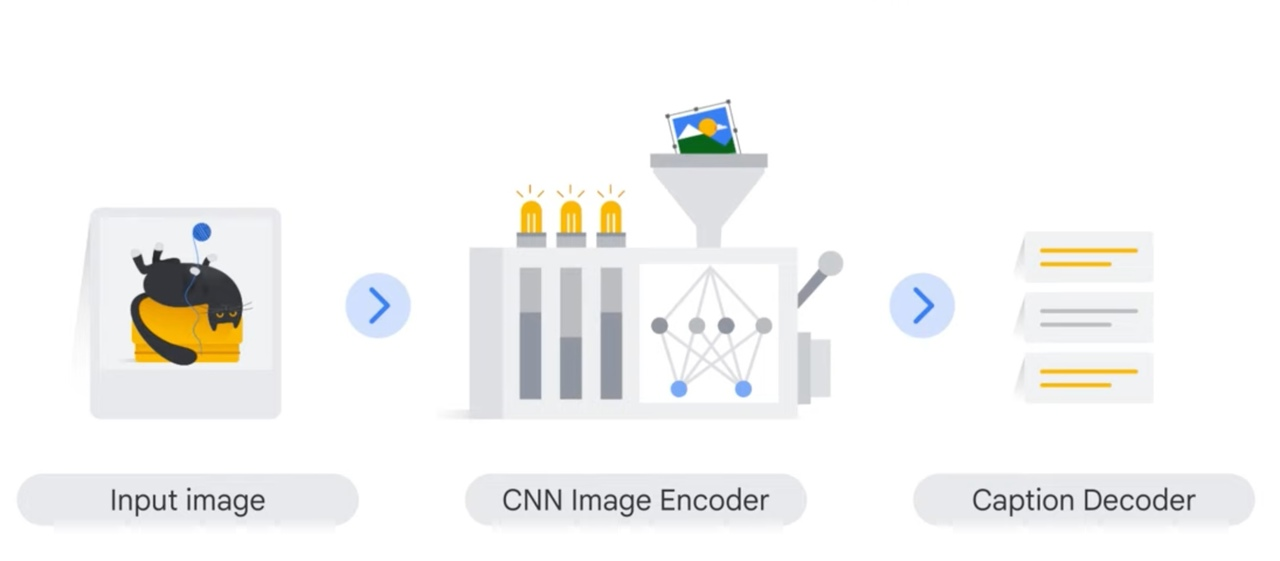
\includegraphics[scale=0.4]{image-captioning-arch.png}
	\caption{Архитектура задачи Image Captioning.}
	\label{fig:image-captioning-arch}
\end{figure}


Кодировщик отвечает за преобразование изображения в компактное представление (вектор признаков), которое сохраняет важную информацию об изображении. Обычно в качестве энкодера используется CNN, такие как ResNet, VGG, Inception, MobileNet или EfficientNet. Эти модели предварительно обучены на больших наборах данных, таких как ImageNet, для извлечения визуальных признаков. В качестве вектора признаков изображения может использоваться выходной слой CNN, но чаще всего это слой перед последним полносвязанным. Также в качестве Image Encoder для извлечения признаков изображения могут быть использованы Vision Transformers (ViT) \cite{vit}. Трансформеры представляют собой архитектуру, основанную на механизме внимания, которая была успешно применена к различным задачам компьютерного зрения, включая генерацию подписей к изображениям. ViT может достичь лучших результатов, чем большинство современных сетей CNN. Однако была разработана модель EfficientNet V2, которая быстрее обучается и обладает меньшей потребностью в ресурсах по сравнению с ViT, но при этом лучше работает со многими задачами компьютерного зрения \cite{efficientnetv2}. Несмотря на высокую производительность, EfficientNet V2 не использует механизм внимания, как ViT, что может быть недостатком в некоторых случаях. Поэтому выбор кодировщика зависит от конкретных требований проекта и условий, в которых будет использоваться модель. В некоторых случаях может быть полезным попробовать обе архитектуры и выбрать ту, которая лучше соответствует задачам и ресурсам.

Декодировщик принимает вектор признаков изображения и генерирует последовательность слов, которая описывает изображение. Декодеры, как правило, основаны на рекуррентных нейронных сетях (RNN), однако современные подходы могут использовать трансформеры. В ранних моделях чаще всего используется LSTM (Long Short-Term Memory) или GRU (Gated Recurrent Unit) для генерации последовательности слов. Одна из основных проблем такого подхода - это то, что RNN имеет фиксированную длину контекста и обрабатывает информацию последовательно. Это означает, что RNN видит только небольшой контекст, поэтому при генерации слов часто забывает старые результаты своей генерации. Так же такой подход не позволяет полностью учесть контекст изображения на каждом этапе генерации. В данном случае выделенные признаки изображения с помощью CNN лишь единожды подаются на вход LSTM блока, так что со временем генерация полностью теряет память о исходном изображении и начинает "додумывать самостоятельно". Для решения этих проблем применяется механизм внимания. В случае image captioning, механизм внимания позволяет сети "обращаться" к различным частям изображения на каждом шаге генерации текста. Таким образом контекст самого изображения не теряется со временем генераций, и механизм внимания позволяет сети сфокусироваться на разных частях изображения с разной степенью "важности" на каждом шаге генерации, что значительно увеличивает качество финального описания. На рисунке \ref{fig:image-captioning-decoder} представлена архитектура декодировщика.


\begin{figure}[ht]
	\centering
	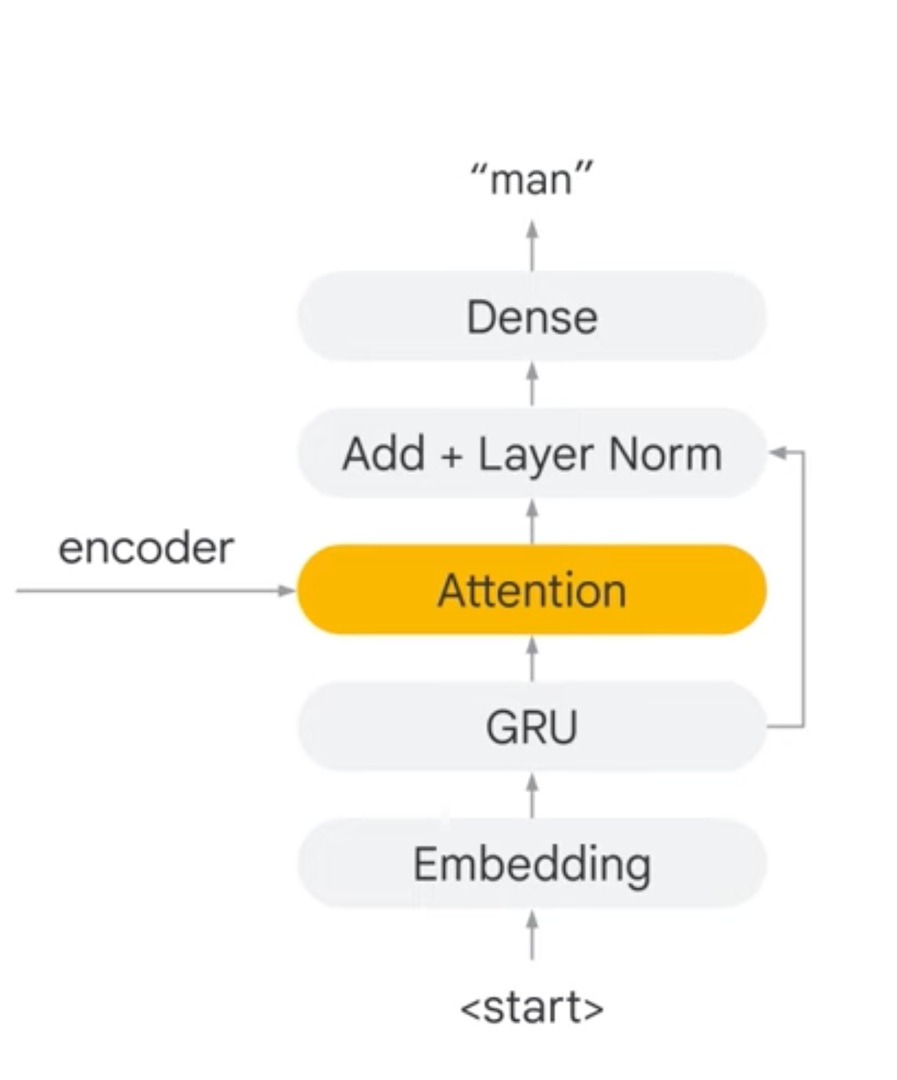
\includegraphics[scale=0.25]{image-captioning-decoder.png}
	\caption{Архитектура декодировщика в задаче Image Captioning.}
	\label{fig:image-captioning-decoder}
\end{figure}

Более современные подходы используют трансформеры, такие как модель Transformer от Vaswani et al.\cite{transformers}. Трансформеры лучше справляются с захватом долгосрочных зависимостей в последовательности слов.

При обучении модели обычно используется кросс-энтропийная функция потерь для сравнения сгенерированных описаний с эталонными в обучающем наборе данных. Для оценки качества генерации используются метрики, такие как BLEU, METEOR и CIDEr.

\subsection{Используемые метрики в задаче классификации}
В задаче классификации для оценки качества моделей машинного обучения используются специальные показатели — метрики.

Для описания метрик используется матрица ошибок классификаций (англ. confusion matrix). Пусть есть два класса и метод, предсказывающий принадлежность каждого объекта одному из классов. В таблице \ref{confusion_matr} представлена матрица ошибок классификации.

\begin{table}[h]
	\centering
	\begin{tabular}{ | l | l | l | }
		\hline
		& $y = 1$ & $y = 0$ \\ \hline
		$\hat{y} = 1$ & True Positive (TP) & False Positive (FP) \\ \hline
		$\hat{y} = 0$ & True Negative (TN) & False Negative (FN) \\ \hline
	\end{tabular}
	\caption{Матрица ошибок классификации.
		$y$ — истинный класс, $\hat{y}$ — результат модели.}
	\label{confusion_matr}
\end{table}

Простейшей метрикой является accuracy — доля правильных ответов:

\begin{equation}
	\label{acc}
	accuracy = \frac{TP + TN}{TP + TN + FP + FN}
\end{equation}

Стоит отметить, что эта метрика может быть применима только на сбалансированном датасете. 


Для оценки качества работы алгоритма на каждом из классов по отдельности вводятся метрики точность (англ. precision)  и полнота (англ. recall): 

\begin{equation}
	\label{precision}
	precision = \frac{TP}{TP + FP}
\end{equation}

\begin{equation}
	\label{recall}
	recall = \frac{TP}{TP + FN}
\end{equation}

Precision — доля объектов, которые классификатор определил как положительные и при этом они действительно являются положительными, а recall — метрика, которая показывает, какую долю положительных объектов из всех объектов положительного класса обнаружила модель. Введение precision не позволяет определять все объекты в один класс, так как в этом случае получается рост FP. Recall показывает способность метода вообще обнаруживать данный класс, а precision — способность отличать этот класс от других. В отличие от accuracy, recall и precision не зависят, от соотношения классов и поэтому могут быть применимы на несбалансированном датасете.

Также существует несколько способов объединить recall и precision в объединенный критерий оценки. Например, F-мера (в общем случае $\ F_\beta$) — среднее гармоническое recall и precision:

\begin{equation}
	\label{acc3}
	\large \ F_\beta = (1 + \beta^2) \cdot \frac{precision \cdot recall}{(\beta^2 \cdot precision) + recall}
\end{equation}

$\beta$ в данном случае определяет вес точности в метрике. 

F-мера достигает максимума при точности и полноте, равными 1, и близка к 0, если один из аргументов близок к 0.


\subsection{Проектирование архитектуры программного продукта (в процессе)}
В 2022 году граждане Российской Федераций столкнулись с трудностями работы с магазинами приложений для смарт-устройств. Так, например, с 24 февраля из российского раздела App Store были удалены почти 7000 мобильных приложений \cite{russia_app}. Поэтому при построении архитектуры приложения был выбран подход к созданию клиент-серверного приложения, которое будет работать практически на любом устройстве (стационарный компьютер, ноутбук, планшет или смартфон). Одним из способов реализации такого подхода является написание telegram  бота. В настоящее время это одно из трендовых направлений в IT сфере. В 2024 году Telegram посещают 900 миллионов человек в месяц. По количеству аудитории он входит в пятерку самых популярных мессенджеров в мире. Выбор в пользу написания телеграм-бота вместо веб-приложения может быть обусловлен рядом факторов, включая удобство использования, скорость разработки, доступность, безопасность, а также гибкость и масштабированность для обработки большого количества пользователей.

За логику, работоспособность и правильное функционирование бота 
отвечает серверная часть (англ. backend), которая скрыта от пользователя. Серверная часть включает в себя:
\begin{itemize}
	\item модуль для обработки запросов от пользователя;
	\item модуль для взаимодействия с обученной моделями классификации для определения категории товара и генерации его описания.
\end{itemize}

В контексте работы с моделями машинного обучения и их применения в системах автономного управления, вынос предсказаний моделей в очередь сообщений может быть полезно для оптимизации работы и повышения устойчивости системы.

Для проектирования, разработки и обучения нейронных сетей использовался следующий стек технологий:
\begin{itemize}
	\item Язык программирования Python — язык общего назначения, с помощью которого можно решать сложные задачи машинного обучения и быстро создавать прототипы для последующей их отладки. Язык гибкий и мультиплатформенный, имеет обширный набор библиотек для искусственного интеллекта. Python удобно использовать для обработки и подготовки обучающих данных.
	\item Pytorch — библиотека глубокого обучения с открытым исходным кодом, написанная на языке Python и созданная на базе Torch. Используется для решения различных задач машинного обучения: компьютерное зрение, NLP, создания и обучения нейронных сетей \cite{pytorch}.
\end{itemize}

Вычисления происходили с использованием аппаратных ускорений на GPU Nvidia Tesla V100 и A100.

Для реализация серверной части был выбран Flask – это небольшой и легкий веб-фреймворк, написанный на языке Python, предлагающий полезные инструменты и функции для облегчения процесса создания веб-приложений с использованием Python \cite{flask}.

Docker — инструмент для создания и запуска контейнеров.

Kubernetes нужен, когда у вас много контейнеров и узлов, которыми нужно управлять. Также Kubernetes подходит, если вам нужна распределенная отказоустойчивая система.


На рисунке \ref{web_arch} представлена структура приложения.


\newpage
\appendix

\section{Приложение 1}
\label{appendix:amount_of_categor2}
\textbf{\large{Распределение данных по категориям второй вложенности.}}

\begin{figure}[hbtp]
	\centering
	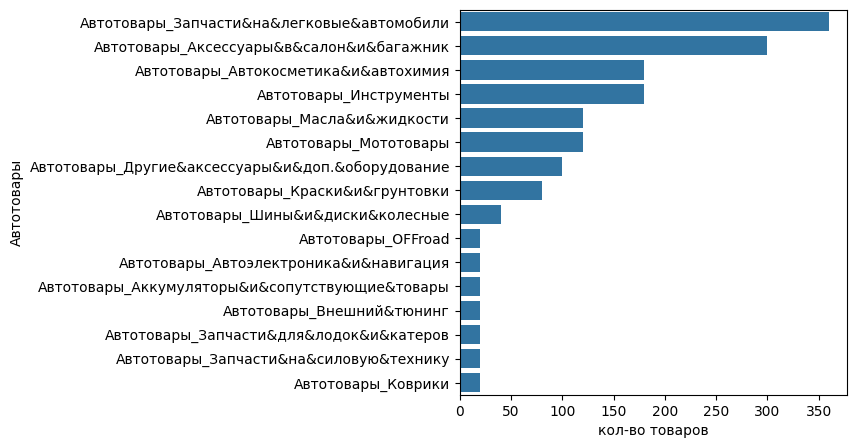
\includegraphics[scale=0.8]{приложения/amount_of_category_Автотовары.png}
	\caption{Распределение данных в категории «Автотовары».}
	\label{fig:amount_of_category_Автотовары}
\end{figure}

\begin{figure}[hbtp]
	\centering
	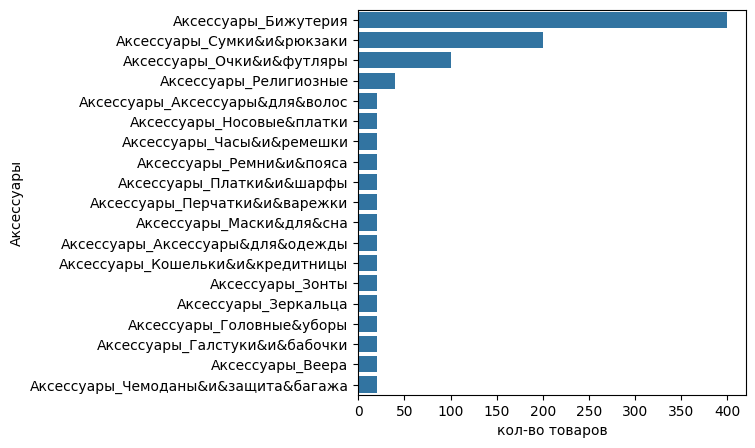
\includegraphics[scale=0.8]{приложения/amount_of_category_Аксессуары.png}
	\caption{Распределение данных в категории «Аксессуары».}
	\label{fig:amount_of_category_Аксессуары}
\end{figure}

\begin{figure}[hbtp]
	\centering
	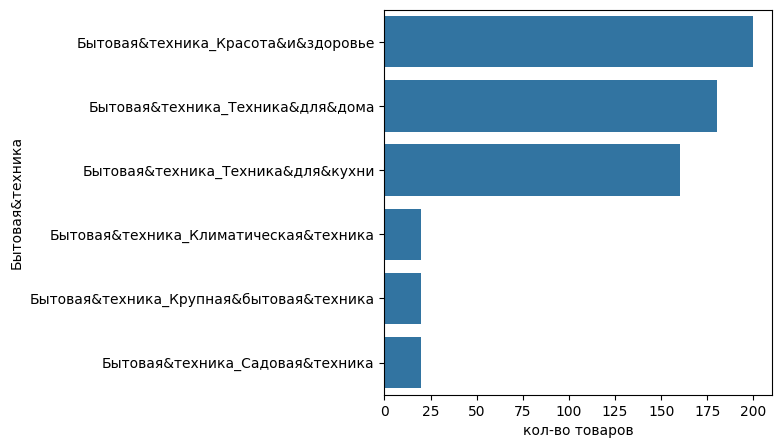
\includegraphics[scale=0.8]{приложения/amount_of_category_Бытовая&техника.png}
	\caption{Распределение данных в категории «Бытовая\&техника».}
	\label{fig:amount_of_category_Бытовая&техника}
\end{figure}

\begin{figure}[hbtp]
	\centering
	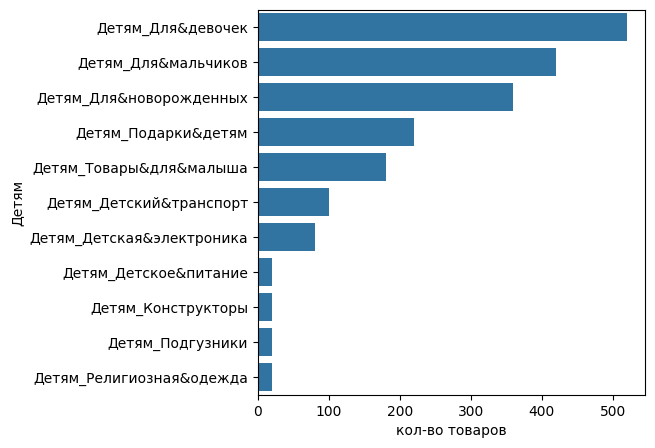
\includegraphics[scale=0.8]{приложения/amount_of_category_Детям.png}
	\caption{Распределение данных в категории «Детям».}
	\label{fig:amount_of_category_Детям}
\end{figure}

\begin{figure}[hbtp]
	\centering
	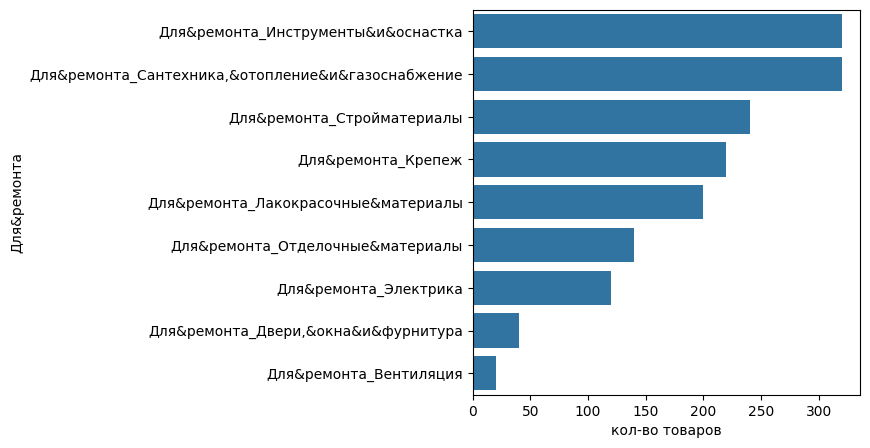
\includegraphics[scale=0.8]{приложения/amount_of_category_Для&ремонта.png}
	\caption{Распределение данных в категории «Для\&ремонта».}
	\label{fig:amount_of_category_Для&ремонта}
\end{figure}

\begin{figure}[hbtp]
	\centering
	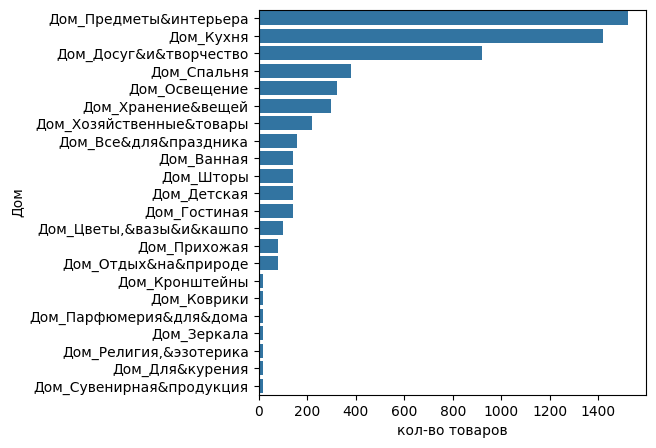
\includegraphics[scale=0.8]{приложения/amount_of_category_Дом.png}
	\caption{Распределение данных в категории «Дом».}
	\label{fig:amount_of_category_Автотовары}
\end{figure}

\begin{figure}[hbtp]
	\centering
	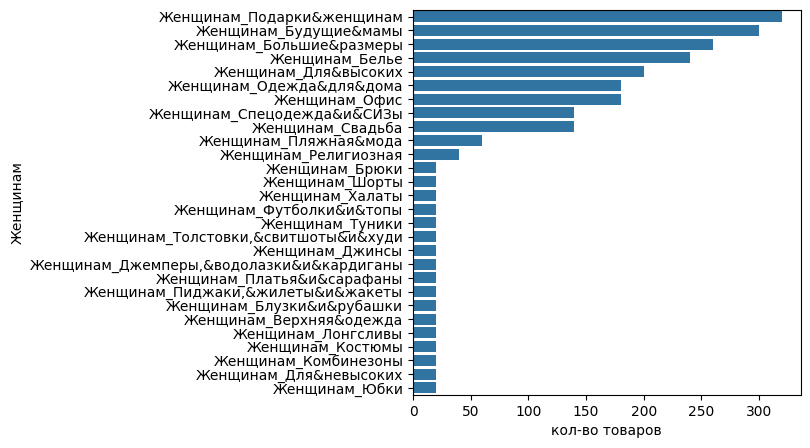
\includegraphics[scale=0.8]{приложения/amount_of_category_Женщинам.png}
	\caption{Распределение данных в категории «Женщинам».}
	\label{fig:amount_of_category_Женщинам}
\end{figure}

\begin{figure}[hbtp]
	\centering
	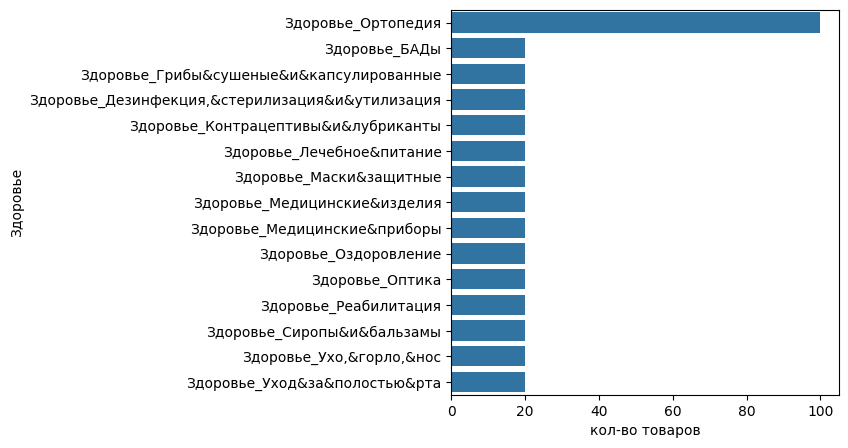
\includegraphics[scale=0.8]{приложения/amount_of_category_Здоровье.png}
	\caption{Распределение данных в категории «Здоровье».}
	\label{fig:amount_of_category_Здоровье}
\end{figure}

\begin{figure}[hbtp]
	\centering
	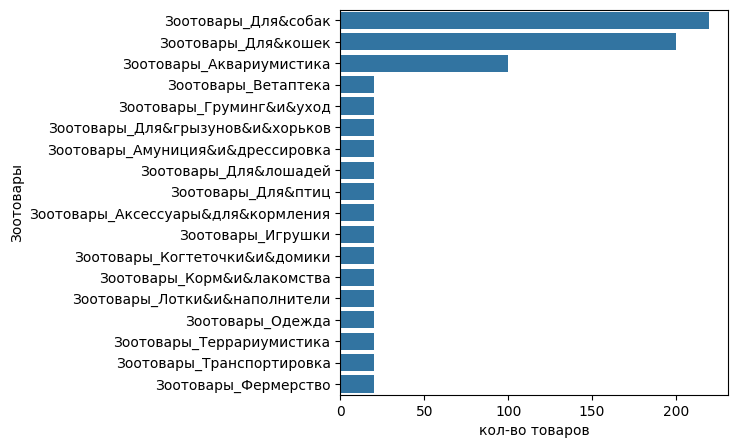
\includegraphics[scale=0.8]{приложения/amount_of_category_Зоотовары.png}
	\caption{Распределение данных в категории «Зоотовары».}
	\label{fig:amount_of_category_Зоотовары}
\end{figure}

\begin{figure}[hbtp]
	\centering
	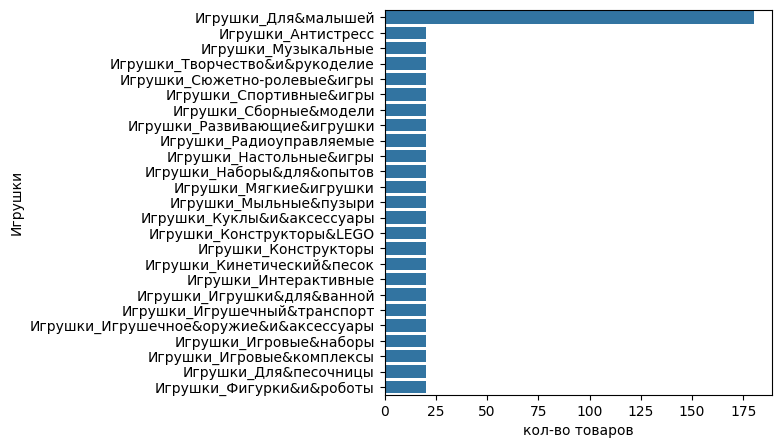
\includegraphics[scale=0.8]{приложения/amount_of_category_Игрушки.png}
	\caption{Распределение данных в категории «Игрушки».}
	\label{fig:amount_of_category_Игрушки}
\end{figure}

\begin{figure}[hbtp]
	\centering
	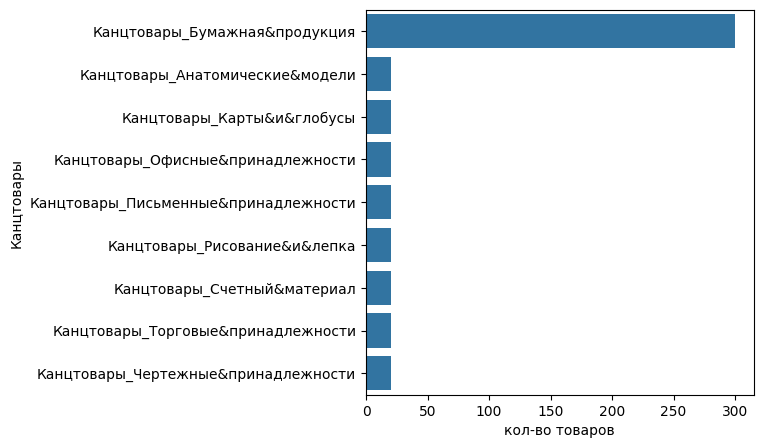
\includegraphics[scale=0.8]{приложения/amount_of_category_Канцтовары.png}
	\caption{Распределение данных в категории «Канцтовары».}
	\label{fig:amount_of_category_Канцтовары}
\end{figure}

\begin{figure}[hbtp]
	\centering
	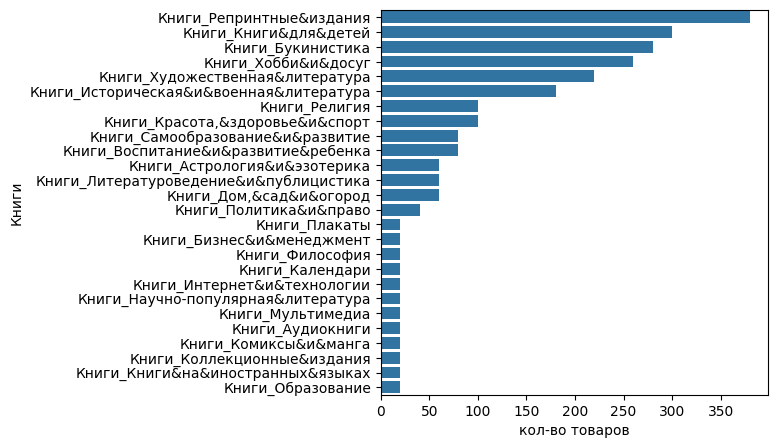
\includegraphics[scale=0.8]{приложения/amount_of_category_Книги.png}
	\caption{Распределение данных в категории «Книги».}
	\label{fig:amount_of_category_Книги}
\end{figure}

\begin{figure}[hbtp]
	\centering
	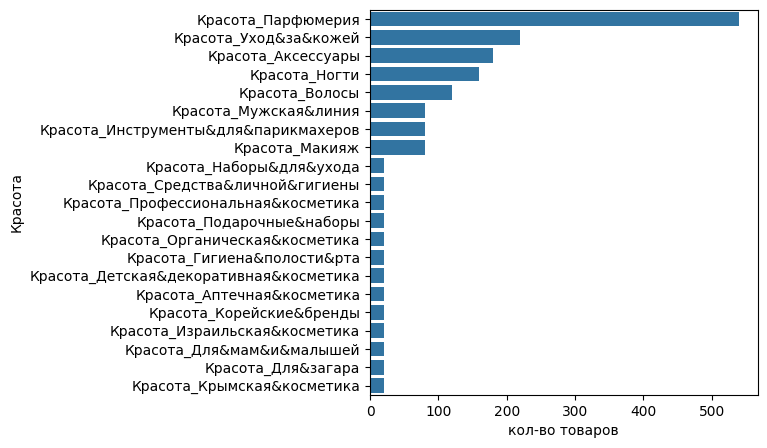
\includegraphics[scale=0.8]{приложения/amount_of_category_Красота.png}
	\caption{Распределение данных в категории «Красота».}
	\label{fig:amount_of_category_Красота}
\end{figure}

\begin{figure}[hbtp]
	\centering
	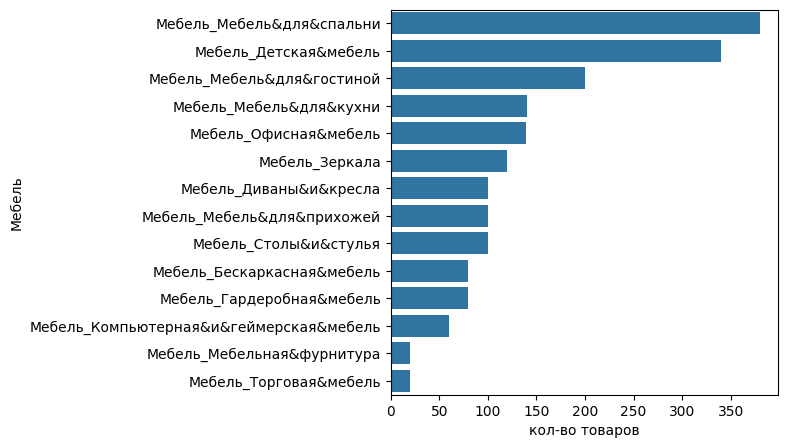
\includegraphics[scale=0.8]{приложения/amount_of_category_Мебель.png}
	\caption{Распределение данных в категории «Мебель».}
	\label{fig:amount_of_category_Мебель}
\end{figure}

\begin{figure}[hbtp]
	\centering
	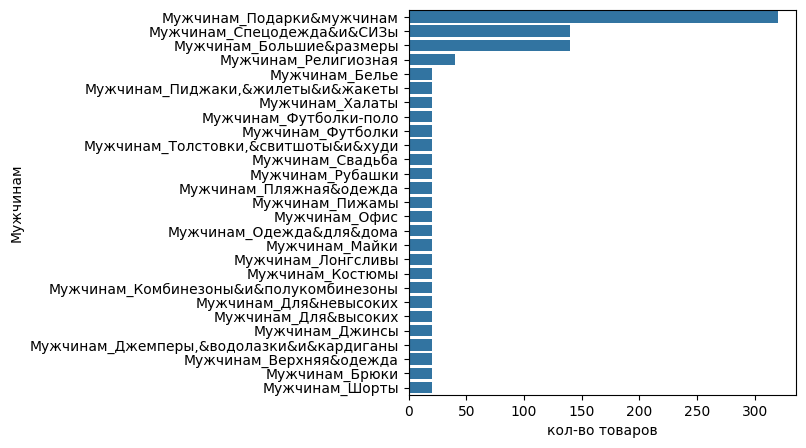
\includegraphics[scale=0.8]{приложения/amount_of_category_Мужчинам.png}
	\caption{Распределение данных в категории «Мужчинам».}
	\label{fig:amount_of_category_Мужчинам}
\end{figure}

\begin{figure}[hbtp]
	\centering
	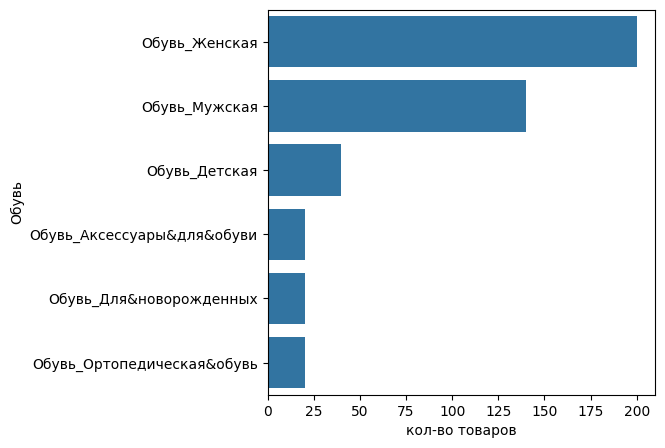
\includegraphics[scale=0.8]{приложения/amount_of_category_Обувь.png}
	\caption{Распределение данных в категории «Обувь».}
	\label{fig:amount_of_category_Обувь}
\end{figure}

\begin{figure}[hbtp]
	\centering
	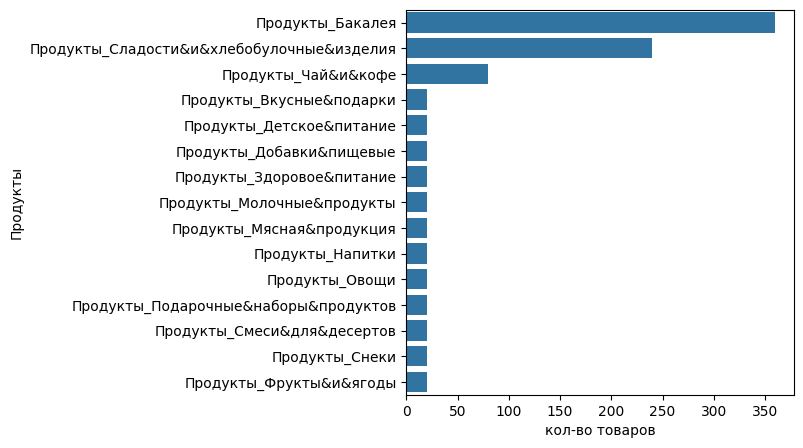
\includegraphics[scale=0.8]{приложения/amount_of_category_Продукты.png}
	\caption{Распределение данных в категории «Продукты».}
	\label{fig:amount_of_category_Продукты}
\end{figure}

\begin{figure}[hbtp]
	\centering
	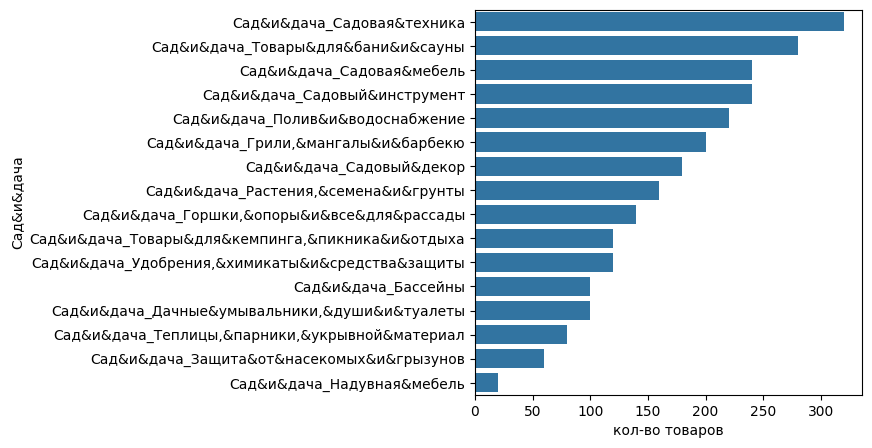
\includegraphics[scale=0.8]{приложения/amount_of_category_Сад&и&дача.png}
	\caption{Распределение данных в категории «Сад\&и\&дача».}
	\label{fig:amount_of_category_Сад&и&дача}
\end{figure}

\begin{figure}[hbtp]
	\centering
	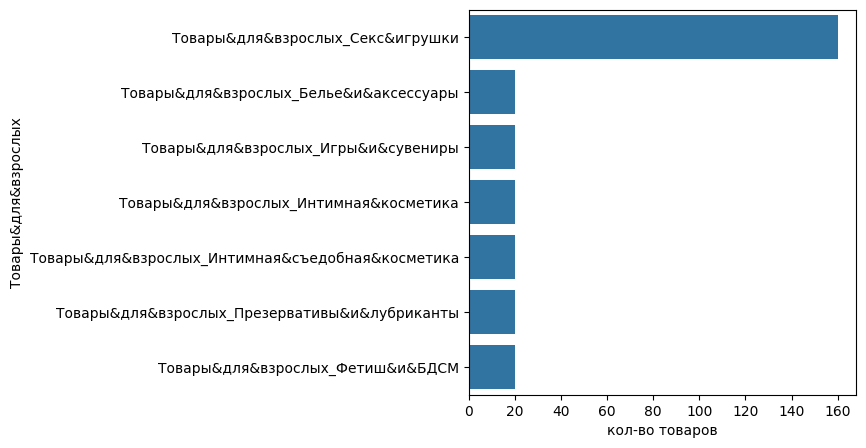
\includegraphics[scale=0.8]{приложения/amount_of_category_Товары&для&взрослых.png}
	\caption{Распределение данных в категории «Товары\&для\&взрослых».}
	\label{fig:amount_of_category_Товары&для&взрослых}
\end{figure}

\begin{figure}[hbtp]
	\centering
	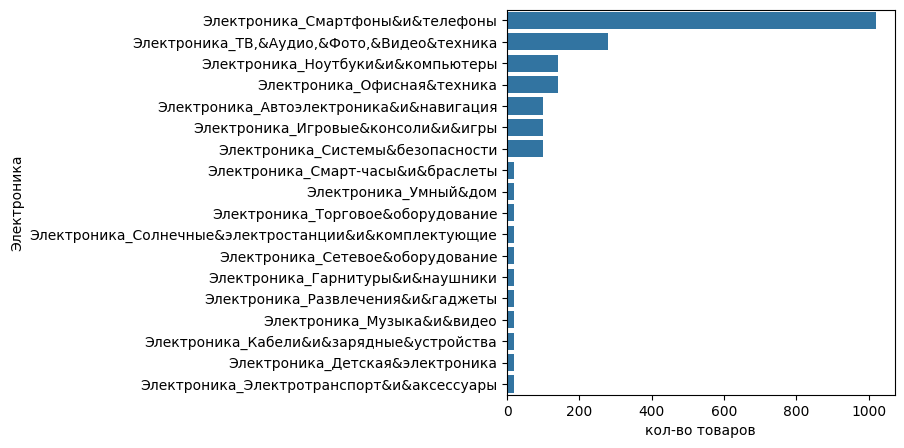
\includegraphics[scale=0.8]{приложения/amount_of_category_Электроника.png}
	\caption{Распределение данных в категории «Электроника».}
	\label{fig:amount_of_category_Электроника}
\end{figure}

\begin{figure}[hbtp]
	\centering
	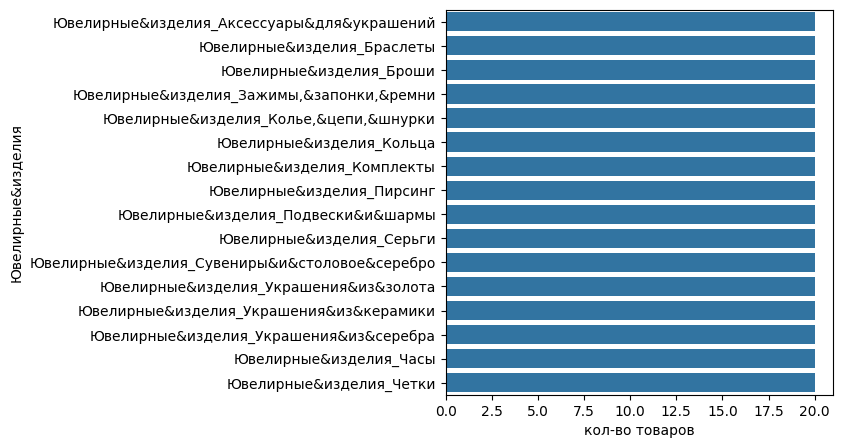
\includegraphics[scale=0.8]{приложения/amount_of_category_Ювелирные&изделия.png}
	\caption{Распределение данных в категории «Ювелирные\&изделия».}
	\label{fig:amount_of_category_Ювелирные&изделия}
\end{figure}

\end{document}
